\documentclass[11pt,a4paper]{article}

\usepackage[margin=2.4cm]{geometry}
\usepackage[T1]{fontenc}
\usepackage{lmodern}
\usepackage{microtype}
\usepackage{amsmath,amssymb}
\usepackage{graphicx}
\usepackage{booktabs}
\usepackage{tabularx}
\usepackage{array}
\usepackage[font=small,labelfont=bf]{caption}
\usepackage{enumitem}
\setlist{noitemsep,topsep=3pt}
\usepackage{xcolor}
\usepackage[numbers,sort&compress]{natbib}
\usepackage{tikz}
\usetikzlibrary{arrows.meta,positioning,fit}
\usepackage[colorlinks=true,linkcolor={blue!50!black},citecolor={blue!50!black},urlcolor={blue!50!black}]{hyperref}

\graphicspath{{../results/figures/}}
\newcommand{\pct}{\,\%}

\title{\textbf{The City Understands the Place:}\\[2pt]
Location Memory from Infrastructure Cameras as a Prior for Autonomous Driving}
\author{Gamzat Gadzhibutaev\thanks{HSE University, Faculty of Economics, Nizhny Novgorod, Russia.
\texttt{gbgadzhibutaev@edu.hse.ru}}}
\date{Working paper --- draft of 29 September 2026}

\begin{document}
\maketitle

\begin{abstract}
A robotaxi perceives a place only while it is there; a fixed camera watches the same place for hours, days and months.
We ask whether this long-term \emph{location memory} is worth anything to an autonomous vehicle, and when it becomes a liability.
Memory is represented as exposure-normalised sufficient statistics with uncertainty---where pedestrians step onto the road, how traffic turns, where vehicles brake hard---and is evaluated in eight steps.
(i)~On two hours of real trajectories from 12 fixed 4K infrastructure cameras in Washington, DC (TGSIM Foggy Bottom), memory built from the first 79 minutes predicts the last 40:
73\pct{} of held-out pedestrian road entries fall inside the 10\pct{} of road area it ranks highest (2.27 bits per entry over a uniform prior), and for vehicles that change direction it picks their heading 3\,s ahead correctly 59\pct{} of the time, against 19\pct{} for area-wide statistics.
(ii)~In a closed-loop occlusion simulation calibrated on the same data, an occlusion-aware planner with 10 hours of memory has 26\pct{} fewer pedestrian collisions at equal trip time (95\pct{} CI 20--33\pct) than a planner that knows only the street's average pedestrian rate, matching perfect knowledge; the benefit grows with the spatial unevenness of pedestrian activity, from 0 to 56\pct.
Two failure modes are severe: stale memory is worse than none, and a live camera that fails silently is the most dangerous state studied. Letting memory only \emph{add} caution, expiring live information with a heartbeat, and a sequential change detector, which notices a moved hotspot within an hour on camera data, remove most of the harm. Letting the vehicle's own sensors take precedence wherever they can see neutralises phantom pedestrians injected into the camera feed, and a fleet audit exposes a camera that silently drops pedestrians within hours.
(iii)~Treating every real vehicle in the data as a potential fleet car shows that a fleet can learn the same memory, but at the pace of equipped cars passing by: at 10\pct{} penetration it needs roughly four times the calendar time of a fixed camera.
(iv)~A full day at an instrumented intersection in Braunschweig (DLR UT) shows that location memory and the live phase of the traffic lights are complementary: together they cut the error of where a vehicle approaching a light will be in 3\,s from 4.8\,m (constant velocity) to 2.7\,m, against 3.9 and 4.2\,m for memory or live phase alone; which light governs which place is itself learned from memory.
(v)~Over four weekday mornings in Athens (pNEUMA, 74{,}405 vehicles), memory built on other mornings is 94--98\pct{} as informative as memory of the same morning at equal volume, and more mornings make it better: location memory transfers across days.
(vi)~A cost-benefit model per block face, with published unit values, shows where this pays: a trusted live camera on a block breaks even at about 3{,}750 robotaxi traversals a day (90\pct{} interval 2{,}340--7{,}450), almost entirely through riders' and vehicles' time rather than avoided crashes, whereas cameras installed for memory alone do not pay where fleets learn their own.
(vii)~At four intersections in Aachen filmed in several sessions on different weekdays (inD), memory of where pedestrians step onto the road built on other days keeps 93\pct{} of the information of same-day memory at equal volume: pedestrian memory, too, transfers across days.
(viii)~On the same data, adding memory features to a gradient-boosting forecast of pedestrians and cyclists cuts the 3\,s position error on a day the model has not seen by 10\pct{} (0.94 to 0.85\,m), and by 15\pct{} for those who change direction.
\end{abstract}

% ============================================================================
\section{Introduction}

Automated vehicles perceive the world with their own sensors, here and now.
At an urban kerb lined with parked cars, this is a hard limit: a pedestrian stepping out between two vans is invisible until the last moment, and a planner that must stop for every pedestrian who \emph{might} be there crawls along the block.
Cities, meanwhile, already operate thousands of fixed cameras, and the number keeps growing.
Vehicle-to-infrastructure (V2I) cooperative perception uses such sensors to share \emph{live} detections with vehicles \citep{yu2022dairv2x,yu2023v2xseq,hu2022where2comm,yu2025univ2x}, and standards for doing so exist \citep{etsi2023cpm,etsi2014ldm}.

A fixed sensor also has something a passing vehicle cannot have: \emph{temporal depth}.
It watches the same place continuously, and over hours and days learns where people cross, how traffic turns, where drivers brake.
A robotaxi may arrive at an intersection for the first time, yet the city may already hold the equivalent of thousands of past passages through it.
In short: the vehicle understands its surroundings; the city understands the place.

This paper asks whether such location memory is worth anything to an autonomous vehicle.
Following a long-standing argument that part of vehicle intelligence can live in the infrastructure \citep{gopalswamy2018iea}, we treat the city's knowledge strictly as a \emph{probabilistic prior} for the vehicle's planner, never as a command: the vehicle's onboard perception keeps the final decision.
The questions are therefore empirical: does memory predict what happens later, does it change driving outcomes, when does it fail, and why would fixed cameras be needed if a fleet of vehicles could learn the same thing?

\paragraph{Contributions.}
\begin{enumerate}
\item A compact, identity-free representation of location memory as exposure-normalised sufficient statistics with empirical-Bayes uncertainty, and a message design whose cost is kilobytes rather than video (\S\ref{sec:memory}).
\item Evidence on real infrastructure-camera data that memory predicts held-out behaviour, together with its honest limits: rare conflicts are statistically invisible in two hours, and signal-driven stop-and-go dominates vehicle prediction error (\S\ref{sec:real}).
\item A closed-loop, rare-event simulation calibrated on the same data that quantifies the safety--time benefit, its dependence on the unevenness of pedestrian activity and on camera coverage, and two failure modes with mitigations (\S\ref{sec:sim}).
\item A fleet-versus-infrastructure comparison on real traffic showing that fleet memory is limited by exposure rather than by quality (\S\ref{sec:fleet}).
\item Evidence from a second, fully instrumented intersection that location memory and live signal phase add up, with the association between places and traffic lights learned from memory (\S\ref{sec:dlr}).
\item Evidence from four weekday mornings in Athens that location memory transfers across days (\S\ref{sec:pneuma}), and from four German intersections that pedestrian memory does too and makes their forecasts better on unseen days (\S\ref{sec:ind}, \S\ref{sec:ind_pred}).
\item A cost-benefit model per block face that combines the simulated effects with published unit values and shows which infrastructure pays off at which robotaxi volume (\S\ref{sec:econ}).
\end{enumerate}
All code, tests and results are in the accompanying repository and reproduce on a laptop in about twenty minutes.

% ============================================================================
\section{Related work}
\label{sec:related}

\paragraph{Cooperative perception and V2X.}
Vehicle--infrastructure datasets \citep{yu2022dairv2x,yu2023v2xseq} and methods \citep{hu2022where2comm,yu2025univ2x} fuse live roadside and onboard observations; V2X-Seq shows that infrastructure trajectories improve forecasting, but with seconds, not months, of history.
ETSI's Collective Perception Service \citep{etsi2023cpm} standardises the exchange of detected objects, and the Local Dynamic Map \citep{etsi2014ldm} already layers static, quasi-static, transient and highly dynamic information---the layered ``city model'' of this paper is an extension of that structure, not a new architecture.
Large deployments are under way, e.g.\ China's vehicle--road--cloud pilots in 20 cities \citep{caixin2024vrc}; a recent survey organises the field \citep{zhang2025survey}.
Closest in spirit is a 2026 vision paper arguing that fixed roadside sensors offer ``temporal depth'' and proposing infrastructure-centric world models \citep{meng2026iwm}; it contains no experiments.

\paragraph{Memory from vehicle fleets.}
Crowd-sourced maps store aggregate driving behaviour per road segment \citep{mobileye_rem}; CHAMP maps pedestrian zones from repeated passes of instrumented vehicles \citep{greer2023champ}; past traversals \citep{you2022hindsight} and neural map priors \citep{xiong2023nmp} improve perception.
These are the natural competitors of infrastructure memory, and \S\ref{sec:fleet} compares the two on the same traffic.

\paragraph{Maps of dynamics.}
Mobile robotics represents place-dependent motion patterns as maps of dynamics \citep{kucner2023mod}; CLiFF-map-based prediction \citep{zhu2023cliff} and its time-conditioned extension \citep{zhu2025stmod} predict long-term human motion. Our flow layer is a discrete CLiFF map.

\paragraph{Occlusion-aware planning.}
Planners place phantom road users in occluded areas, which is safe but conservative; V2X information reduces the uncertainty and the conservatism \citep{zhang2024occlusion}. Emergence probabilities of hidden pedestrians have been estimated from the current context \citep{koc2021emergence}; we estimate them from long-term infrastructure history.

\paragraph{Safety analytics from infrastructure.}
Commercial systems accumulate near-miss statistics from existing cameras \citep{derq_insight}, roadside LiDAR supports post-hoc safety auditing \citep{shang2026auditing}, and long-term roadside observations have been used to learn realistic, location-specific driving environments for AV testing \citep{yan2023neuralnde}. In these works memory serves agencies or test engineers; here it serves the vehicle's planner.

% ============================================================================
\section{Location memory}
\label{sec:memory}

\begin{figure}[t]
\centering
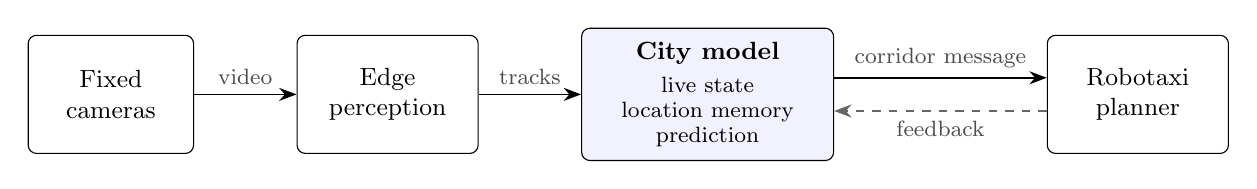
\begin{tikzpicture}[
  box/.style={draw, rounded corners=3pt, align=center, minimum height=1.5cm, inner sep=5pt, font=\small},
  arr/.style={-{Stealth[length=2.2mm]}, semithick},
  lab/.style={font=\footnotesize, align=center, text=black!70}]
\node[box, minimum width=2.1cm] (cam) {Fixed\\cameras};
\node[box, right=1.3cm of cam, minimum width=2.3cm] (edge) {Edge\\perception};
\node[box, right=1.3cm of edge, minimum width=3.2cm, fill=blue!5] (cm) {\textbf{City model}\\[1pt]{\footnotesize live state}\\[-2pt]{\footnotesize location memory}\\[-2pt]{\footnotesize prediction}};
\node[box, right=2.7cm of cm, minimum width=2.3cm] (car) {Robotaxi\\planner};
\draw[arr] (cam) -- node[lab, above] {video} (edge);
\draw[arr] (edge) -- node[lab, above] {tracks} (cm);
\draw[arr] ([yshift=6pt]cm.east) -- node[lab, above] {corridor message} ([yshift=6pt]car.west);
\draw[arr, dashed, black!60] ([yshift=-6pt]car.west) -- node[lab, below] {feedback} ([yshift=-6pt]cm.east);
\end{tikzpicture}
\caption{Architecture. Video never leaves the edge; the city model keeps a live state, a long-term location memory and short-term predictions, and sends each vehicle only the part relevant to its corridor, with an age and a confidence. The vehicle treats it as a prior.}
\label{fig:arch}
\end{figure}

\paragraph{Observations.}
Fixed sensors observe tracks $o=(\text{id}, t, \mathbf{x}, \mathbf{v}, \text{class})$ in a common map frame.
Memory is kept per grid cell $c$ (1\,m) and per lane or crosswalk segment $r$, and consists of \emph{sufficient statistics}, never raw trajectories or identities: long-term mobility traces are re-identifiable even when anonymised \citep{demontjoye2013unique}, while per-cell counts are not.

\paragraph{Layers.}
For each road-user class (pedestrian, micro-mobility, vehicle) the memory stores
(a)~\emph{occupancy and exposure}: agent-seconds and distinct passages per cell, used to normalise every rate;
(b)~a \emph{flow field}: for 8 heading bins per cell, the count, mean direction and mean speed of moving samples (a discrete CLiFF map \citep{zhu2023cliff});
(c)~\emph{manoeuvre transitions}: counts $T_c[b_0,b_3]$ of heading bin now versus 3\,s later;
(d)~vehicle \emph{speed quantiles} per cell;
and events:
(e)~\emph{pedestrian emergence}, the first appearance of a pedestrian on the road after stitching tracker fragments;
(f)~\emph{hard braking}, sustained deceleration $\le -3.5$\,m/s$^2$ for $\ge 0.5$\,s at $\ge 3$\,m/s;
(g)~vehicle--pedestrian \emph{conflicts}, time-to-collision \citep{hayward1972ttc} $\le 1.5$\,s under constant velocity with a three-disc vehicle footprint.

\paragraph{Rates with uncertainty.}
For segment $r$ with $k_r$ events in $n_r$ passages, the per-passage probability has an empirical-Bayes posterior
\begin{equation}
p_r \sim \mathrm{Beta}\bigl(m\bar p + k_r,\; m(1-\bar p) + n_r - k_r\bigr), \qquad \bar p = \textstyle\sum_r k_r / \sum_r n_r ,
\end{equation}
with prior strength $m$ chosen by beta-binomial marginal likelihood, which shrinks sparsely observed segments towards the pooled rate.
Manoeuvre distributions are shrunk the same way towards area-wide transitions, $\hat p(b_3\mid c,b_0) = \bigl(T_c[b_0,b_3] + \alpha\, \bar p(b_3\mid b_0)\bigr)/\bigl(\sum_b T_c[b_0,b] + \alpha\bigr)$ with $\alpha=2$, and the emergence intensity $\lambda(\mathbf{x})$ is a Gaussian-smoothed ($\sigma = 1.5$\,m) count per unit area and time over the observed road area.

\paragraph{The message.}
Layers are split by how often they change.
The memory tile for a vehicle's corridor (90\,m long, 24\,m wide, six one-byte layers) is sent once and cached; only the live object list and short-term predictions stream at 10\,Hz.
A seemingly compact alternative---a dense $200\times200$\,m tensor at 0.5\,m resolution with ten channels at 10\,Hz---costs about 128\,Mbit/s, as much as raw video; ``not video'' is not automatically cheap.

% ============================================================================
\section{Part 1: does memory predict the place?}
\label{sec:real}

\paragraph{Data.}
TGSIM Foggy Bottom \citep{tgsim_fb} was recorded by 12 stationary 4K infrastructure cameras covering four intersections, crosswalks and the road segments between them in Washington, DC, over two hours of a weekday afternoon at 10\,Hz, with all road-user classes and one SAE Level~3 test vehicle.
After stitching pedestrian fragments (a track starting $\le 1$\,s after another ended within 2\,m of its constant-velocity extrapolation; 15{,}307 $\to$ 14{,}237 tracks) and removing tracks shorter than 1\,s, 2.48\,M points remain: 11{,}521 pedestrian and 4{,}930 vehicle tracks, with 11{,}510 pedestrian emergences, 1{,}424 hard-braking onsets and 36 conflicts.

\paragraph{Protocol.}
Memory is built from the first 79 minutes and evaluated on the last 40, which it never saw; blocked three-fold cross-validation holds out each 40-minute block once.
The baseline is always what a vehicle arriving for the first time would know: a uniform distribution over the road area, or area-wide pooled statistics.
Scores are information gain in bits, capture curves, Brier skill, ROC AUC and top-1 accuracy, with bootstrap confidence intervals; prediction hyper-parameters are tuned on a separate validation split.

\begin{figure}[t]
\centering
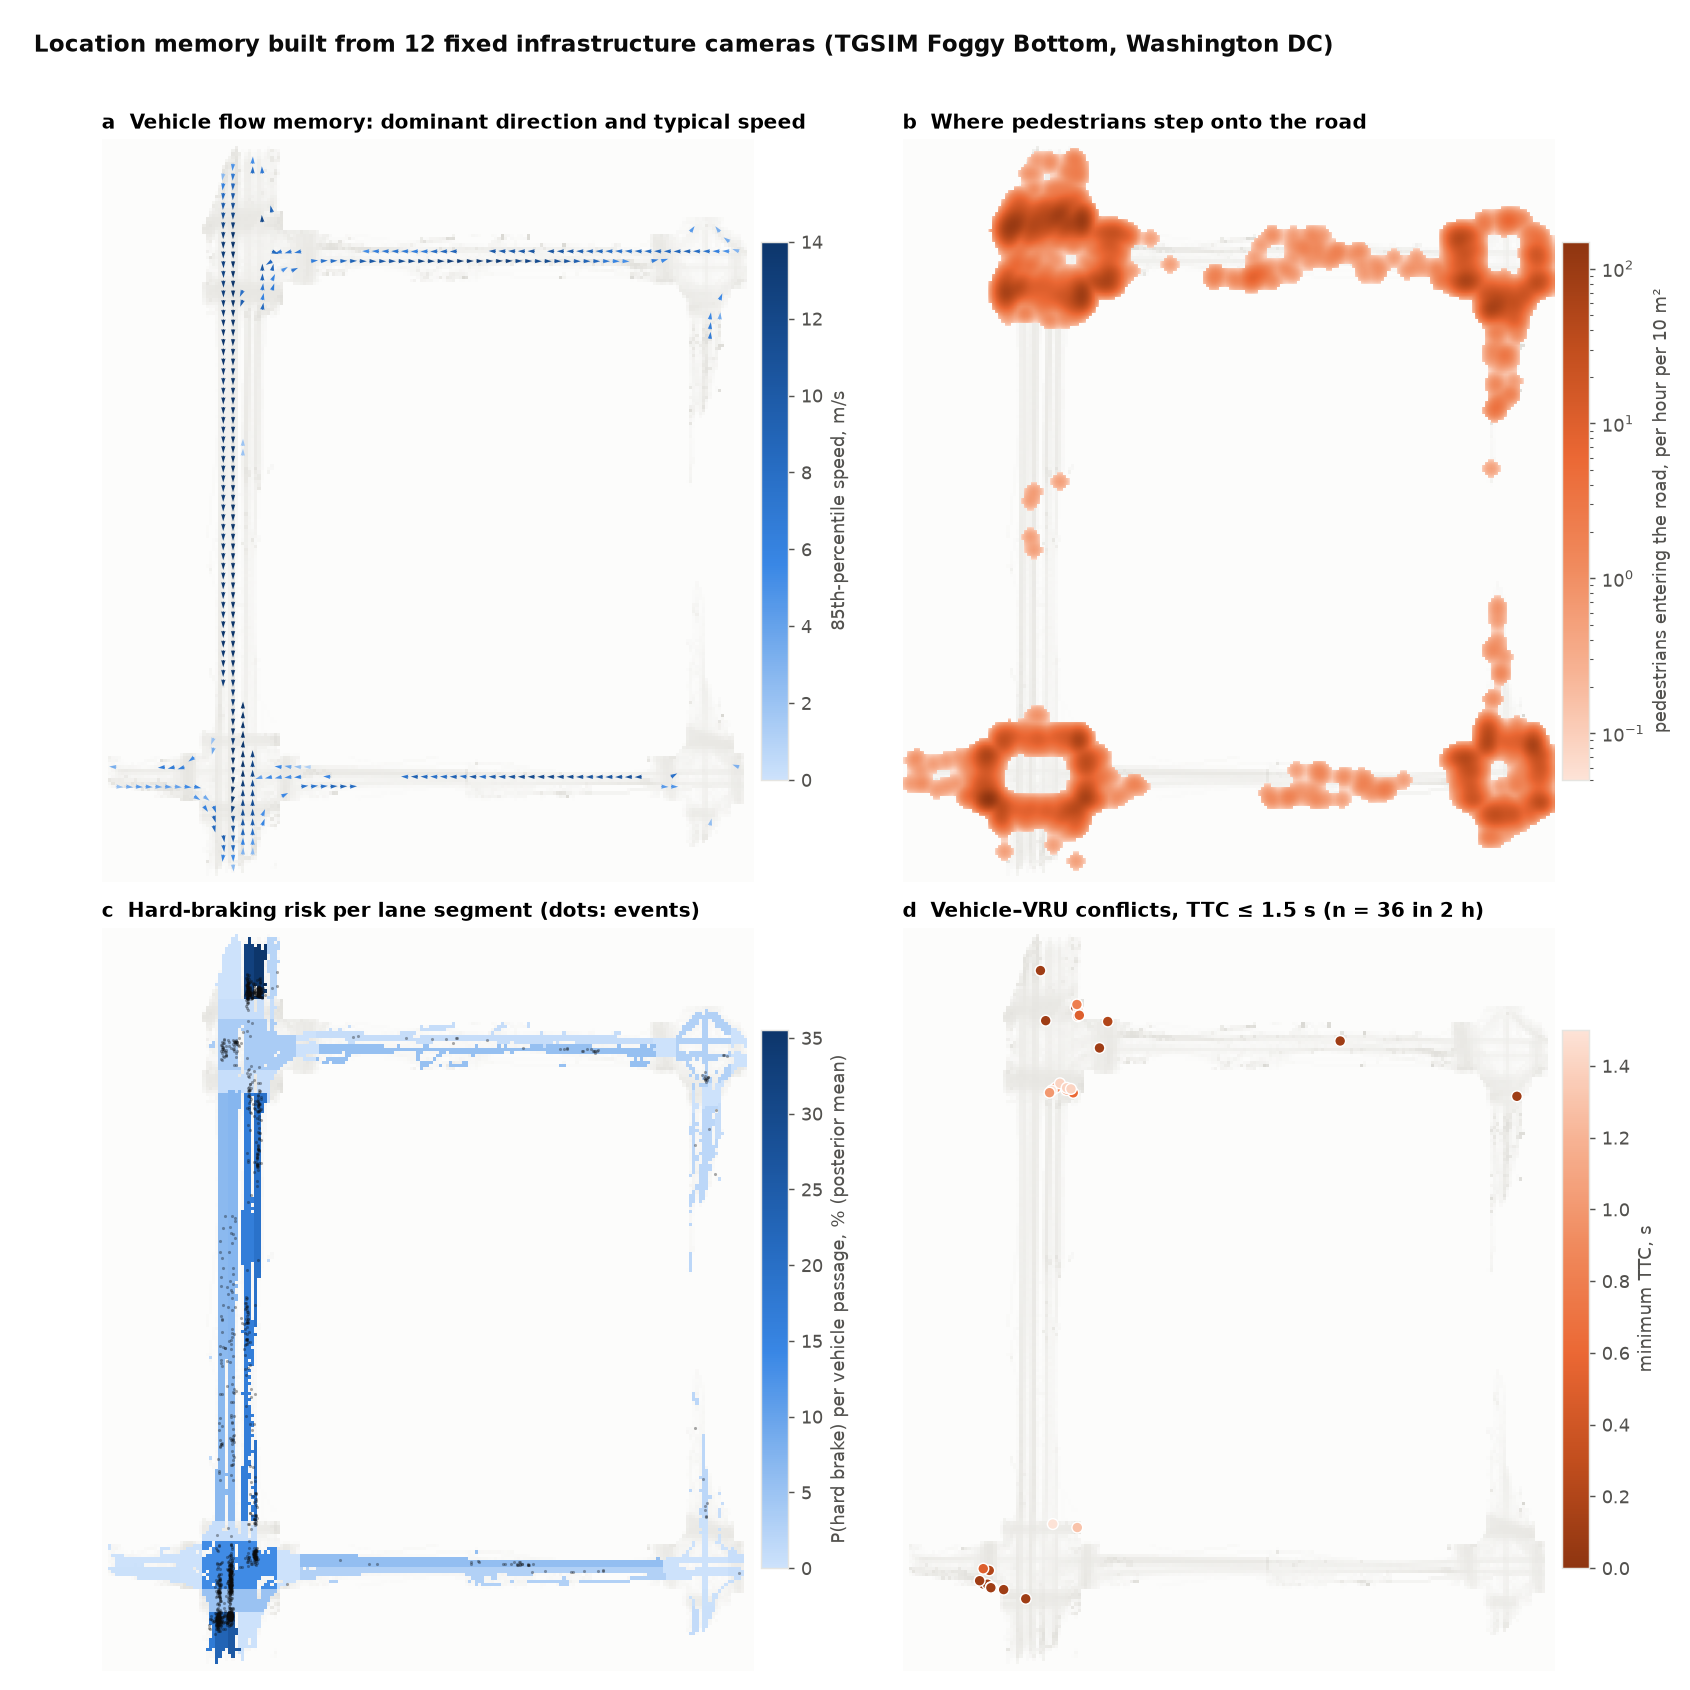
\includegraphics[width=0.74\linewidth]{fig1_location_memory.png}
\caption{Location memory built from the first 79 minutes: (a) vehicle flow and typical speed, (b) where pedestrians step onto the road, (c) posterior hard-braking probability per lane segment, (d) the 36 vehicle--pedestrian conflicts of the two hours.}
\label{fig:memory}
\end{figure}

\begin{table}[t]
\centering\small
\caption{Part 1: memory versus the location-agnostic prior on the held-out 40 minutes.}
\label{tab:real}
\begin{tabularx}{\linewidth}{>{\raggedright\arraybackslash}X >{\raggedright\arraybackslash}p{5.6cm} >{\raggedright\arraybackslash}p{2.6cm}}
\toprule
Question (held-out sample) & Memory & No memory \\
\midrule
Where do pedestrians step onto the road? (4{,}334 entries) & 73\pct{} in the top 10\pct{} of area; $+2.27$ bits [2.22, 2.31] & 10\pct{} (uniform) \\
\quad \ldots outside crosswalks (799) & 42\pct{} in the top 10\pct; $+0.84$ bits [0.72, 0.97] & 10\pct \\
Which lane segments produce hard braking? (9{,}905 passages) & AUC 0.85; Brier skill $+0.08$ & pooled rate 5.7\pct \\
Heading in 3\,s of vehicles that change direction (17{,}154) & 59\pct{} correct; $P(\text{true}) = 0.52$ & 19\pct; 0.33 \\
3\,s position error of turning vehicles (1{,}110) & 5.22\,m ($-18\pct$ [$-16$, $-20$]) & 6.38\,m (constant velocity) \\
Conflict per pedestrian passage (5{,}601; 8 events) & Brier skill $-0.005$ (no gain) & pooled rate 0.23\pct \\
\bottomrule
\end{tabularx}
\end{table}

\paragraph{Where people step onto the road.}
Figure~\ref{fig:memory} shows the memory; Table~\ref{tab:real} and Figure~\ref{fig:heldout} summarise the held-out scores.
Seventy-three percent of held-out pedestrian entries fall inside the 10\pct{} of road area that memory ranks highest, 2.27 bits per entry better than a uniform prior; cross-validation folds agree (2.27--2.44 bits).
The harder case---entries outside crosswalks, between parked or queued cars---is still captured four times better than uniform.
The learning curve is not saturated: 5, 10, 20, 40 and 79 minutes of history give 1.46, 1.73, 1.93, 2.15 and 2.27 bits.

\begin{figure}[t]
\centering
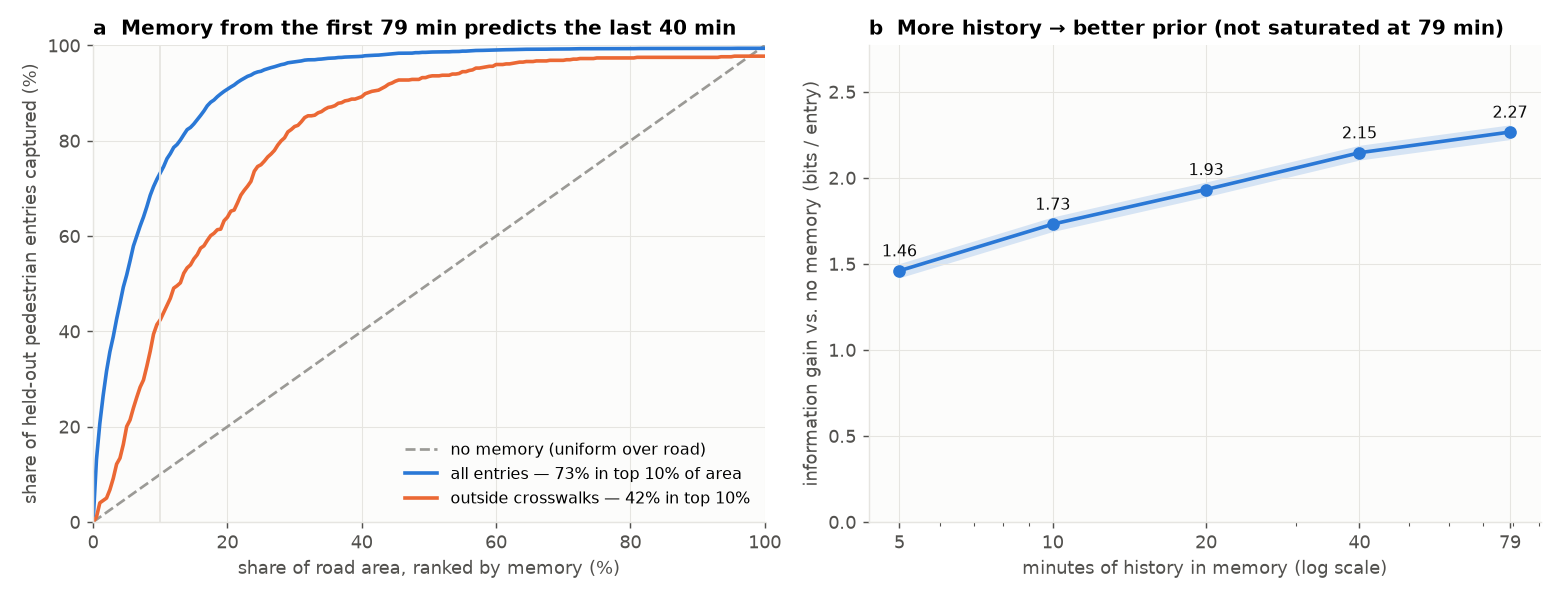
\includegraphics[width=0.95\linewidth]{fig2_emergence_heldout.png}
\caption{(a) Share of held-out pedestrian road entries captured by the top-ranked share of road area. (b) Information gain versus minutes of history.}
\label{fig:heldout}
\end{figure}

\paragraph{How traffic behaves there.}
Segment-level hard-braking rates are calibrated and discriminative (AUC 0.85; cross-validated Brier skill $+0.085$ to $+0.115$).
Memory also knows the manoeuvre distribution of each place: for vehicles whose heading bin changes within 3\,s it predicts the new heading correctly 59\pct{} of the time, versus 19\pct{} with area-wide transitions (Figure~\ref{fig:prediction}a); for pedestrians the gain is smaller (0.10 bits per sample).
Used deterministically, the flow prior reduces the 3\,s error of turning vehicles by 18\pct{} but cannot improve straight-going ones: a single rollout must commit to one manoeuvre, so the planner should receive the distribution rather than one guess (Figure~\ref{fig:prediction}b).

\begin{figure}[t]
\centering
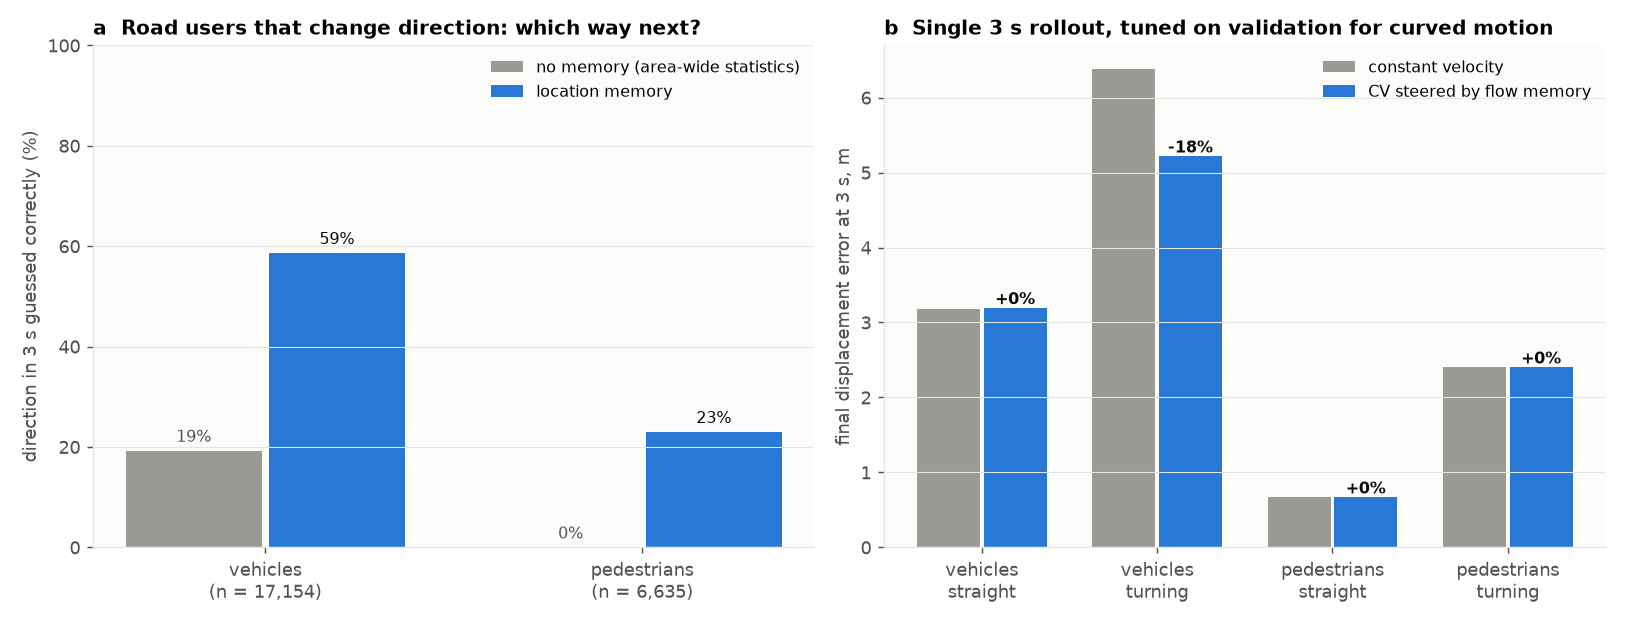
\includegraphics[width=0.95\linewidth]{fig4_prediction.png}
\caption{(a) Heading 3\,s ahead for road users that change direction. (b) Final displacement error of a single 3\,s rollout steered by the flow memory, tuned on validation data for curved motion.}
\label{fig:prediction}
\end{figure}

\paragraph{What memory does not know.}
Two negatives are informative.
First, vehicle--pedestrian conflicts are rare---36 in two hours, eight in the test window---and a per-crosswalk conflict prior is indistinguishable from the pooled rate. Rare safety events need weeks to months of memory, which is an argument for long-term infrastructure memory, not against it.
Second, 3.2 of the 3.3\,m constant-velocity error of vehicles at 3\,s is longitudinal: stop-and-go at signals. A memory of the place cannot know the current signal phase, which only live data can supply.

\paragraph{Occlusion and bandwidth.}
Treating every moving vehicle as a virtual robotaxi with a roof sensor and 2-D line of sight blocked by other vehicles (with stopped vehicles keeping their orientation), 10.4\pct{} of 3{,}042 encounters with a pedestrian on or entering the vehicle's path start hidden, and in 3.8\pct{} the infrastructure knows about the pedestrian at least 1\,s earlier (lower bound with buses and trucks as the only occluders: 0.7\pct{} and 0.3\pct). These numbers are strongly underestimated because the data contain neither sidewalks nor buildings.
For the real test vehicle at one such moment, the corridor tile is 2.7\,KB and the live object list about 12\,kbit/s, against roughly 180\,Mbit/s of raw 4K video from the 12 cameras.

% ============================================================================
\section{Part 2: does memory help a robotaxi drive?}
\label{sec:sim}

\subsection{Simulation calibrated on the real block}

\paragraph{Scene.}
A 90\,m block with a dense parked row (cars 4.3--5.2\,m, gaps mostly 0.6--2\,m); the robotaxi drives in the adjacent lane with 1\,m lateral clearance at up to 25\,mph (11.2\,m/s).
Pedestrians step out between parked cars \emph{where and how often they did in TGSIM}: the emergence profile $\lambda(x)$ is the smoothed histogram of the 99 real mid-block emergences on the block between two of the intersections (about 50 per hour, peak 3.3 times the mean), and walking speeds follow the real distribution of those pedestrians (median 1.49\,m/s, 90th percentile 2.25\,m/s).
Ninety percent of pedestrians are attentive (they wait if the car is less than 3\,s away), ten percent step out without looking, and nobody walks into the side of a passing car.

\paragraph{Vehicle and perception.}
A roof sensor sees a pedestrian when its 2-D sight line clears the parked row; the planner reacts after $t_r = 0.25$\,s of continuous visibility and can brake at $a_e = 7$\,m/s$^2$.
An optional infrastructure camera reports pedestrians approaching the kerb with 0.3\,s latency.

\paragraph{Planner.}
A pedestrian leaving the occlusion edge at distance $d$ ahead of the bumper is unavoidable if the car can neither stop before it nor pass before the pedestrian reaches its path:
$v T_p < d < v t_r + v^2/(2a_e)$, where $T_p$ is the pedestrian's time from the occlusion edge to the vehicle's swath.
With emergences at rate $\lambda(x)$ per metre and second, the car is exposed at $x$ for
\begin{equation}
b(v) = \max\bigl(0,\; t_r + v/(2a_e) - T_p\bigr)
\end{equation}
seconds, and minimising $\int \mathrm{d}x/v + w \int \lambda\, b(v)\, \mathrm{d}x$ pointwise yields the target speed
\begin{equation}
v^\ast(x) = \min\Bigl(v_{\max},\; \max\bigl(v_{\text{wc}},\; \sqrt{2a_e / (w\,\lambda(x))}\bigr)\Bigr), \qquad v_{\text{wc}} = 2a_e (T_p - t_r),
\label{eq:vstar}
\end{equation}
smoothed backwards for comfortable deceleration; $v_{\text{wc}}$ (9\,km/h here) is the worst-case speed at which $b=0$.
All planners share this model and the exchange rate $w$ between time and risk; they differ \emph{only} in the intensity map $\lambda$ they believe (Table~\ref{tab:planners}).
The no-memory planner knows the street's true \emph{average} rate, so any gain measures the value of knowing \emph{where}, not \emph{how many}.

\begin{table}[t]
\centering\small
\caption{Planners in the simulator. All use Eq.~\eqref{eq:vstar} with the same $w$.}
\label{tab:planners}
\begin{tabularx}{\linewidth}{lX}
\toprule
Planner & Believed pedestrian intensity \\
\midrule
Worst case & a pedestrian may step out anywhere at any time ($v=v_{\text{wc}}$ along the parked row) \\
No memory & the street's true mean rate, uniform along the block \\
Location memory & estimated from $H$ hours of simulated camera observation (10\,h: 448 events, with sampling noise) \\
Memory, adds caution only & memory, but never faster than the no-memory planner \\
Perfect memory & the true $\lambda(x)$ (upper bound) \\
$+$ live camera & covered sections believed clear; approaching pedestrians reported \\
\bottomrule
\end{tabularx}
\end{table}

\paragraph{Rare-event design.}
Each episode contains exactly one pedestrian, who reaches the kerb within a window of $W=11$\,s around the robotaxi's nominal arrival at that spot. Per-traversal rates are
\begin{equation}
\mathbb{E}[\text{events per traversal}] = \Lambda W \bigl[p_i\, P(\text{event}\mid\text{inattentive}) + (1-p_i)\, P(\text{event}\mid\text{attentive})\bigr],
\end{equation}
with $\Lambda$ the street's emergence rate and $p_i = 0.1$.
Every configuration runs 30{,}000 inattentive and 3{,}000 attentive episodes, identical across planners (common random numbers); differences carry paired-bootstrap intervals.
A unit test checks that the worst-case planner never hits a pedestrian walking at the planner's design speed, i.e.\ that planner model and simulator agree.
Because the inattentive share is a free parameter, \emph{absolute} collision rates are not calibrated to crash statistics; only comparisons between planners are meaningful.

\subsection{Results}

\begin{figure}[t]
\centering
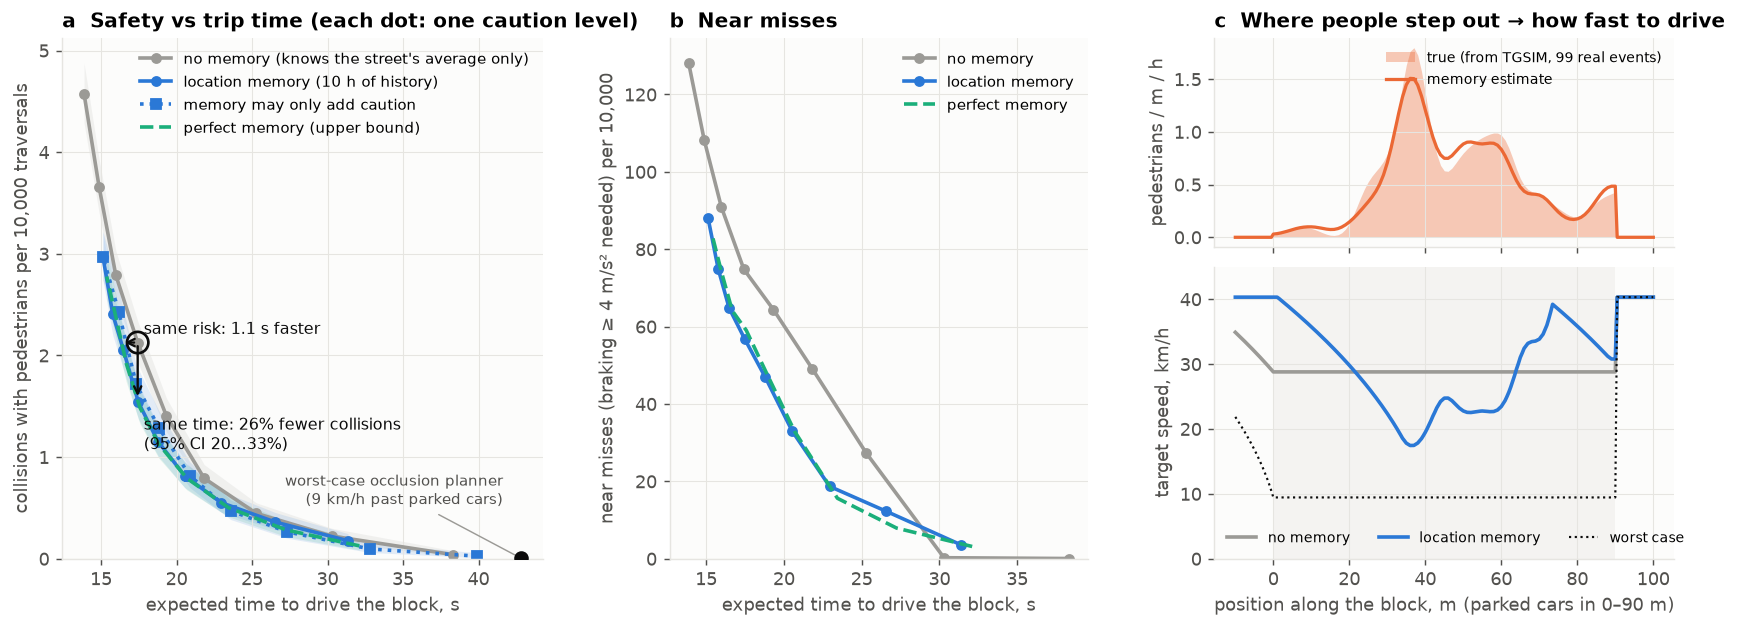
\includegraphics[width=\linewidth]{sim1_pareto.png}
\caption{(a) Collisions versus trip time; each dot is one caution level. The arrows compare planners at the circled no-memory operating point. (b) Near misses (braking $\ge 4$\,m/s$^2$ needed). (c) Real emergence profile, memory estimate and resulting target speeds.}
\label{fig:pareto}
\end{figure}

\paragraph{Memory moves the safety--time frontier.}
At the trip time of the no-memory planner at a human-like caution level, the planner with 10 hours of memory has 26.5\pct{} fewer collisions (95\pct{} CI 20.1--32.8\pct), equal to perfect memory (26.7\pct); at equal risk it is 1.1\,s (6\pct) faster over the block, and near misses also drop (Figure~\ref{fig:pareto}).
It slows to 17\,km/h at the hotspot and drives 40\,km/h where nobody steps out, instead of a uniform 29\,km/h; the worst-case planner crawls at 9\,km/h.
The benefit saturates at about 4 hours of history ($\approx$\,200 observed emergences); 15 minutes of history is sometimes worse than no memory (Figure~\ref{fig:context}b).

\paragraph{It pays off where activity is uneven.}
Under a risk proportional to $\lambda v$ and a time proportional to $1/v$, the optimal speed scales as $\lambda^{-1/2}$ and the achievable risk--time product relative to ignoring location is $(\mathbb{E}\sqrt{\lambda})^2/\mathbb{E}\lambda$.
We use $1-(\mathbb{E}\sqrt{\lambda})^2/\mathbb{E}\lambda$ as a heterogeneity index of a place.
Redistributing the same total pedestrian rate along the block, the collision reduction at equal time grows monotonically with this index: 0\pct{} for a uniform street, 27\pct{} for the real block (index 18\pct), 56\pct{} when the peak is ten times the mean (Figure~\ref{fig:context}c).
The index is a predictor rather than a bound---the real planner's risk has an offset $v_{\text{wc}}$---but it is measurable from a few hours of camera data and tells a city where memory is worth deploying.

\paragraph{Live cameras are the bigger lever.}
With a camera covering the whole block, collisions fall by about 99\pct{} and the block is driven 3\,s faster; memory then adds nothing.
With partial coverage memory still reduces collisions by 10--36\pct, depending on how uneven the \emph{uncovered} part is (Figure~\ref{fig:context}a).

\begin{figure}[t]
\centering
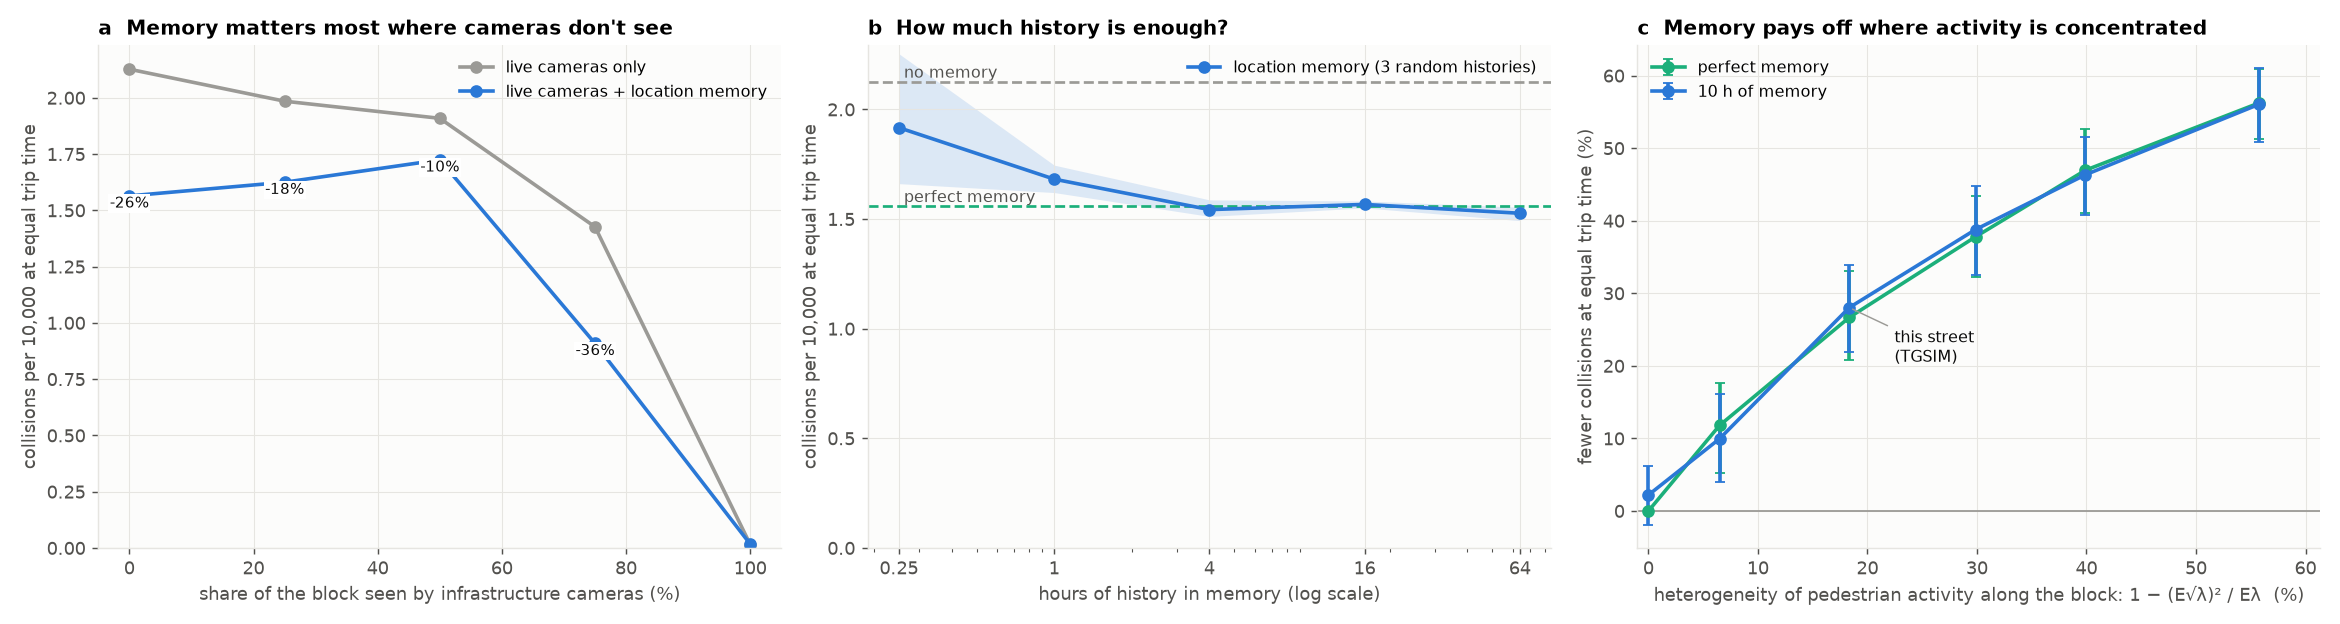
\includegraphics[width=\linewidth]{sim2_coverage_history.png}
\caption{(a) Collisions at equal trip time versus the share of the block seen by cameras. (b) Versus hours of history. (c) Collision reduction versus the heterogeneity of pedestrian activity; bands are 95\pct{} paired-bootstrap intervals.}
\label{fig:context}
\end{figure}

\paragraph{Failure modes.}
Two failures are severe (Figure~\ref{fig:failure}).
When the hotspot moves 21\,m to the quietest part of the block and memory does not know, memory trusted in both directions drives fast exactly where people now step out: 2.52 collisions per 10{,}000 traversals versus 2.00 without memory. A caution floor barely helps (2.44). If memory may only \emph{add} caution, the stale memory still beats no memory (1.62, at the cost of 1.4\,s); with correct memory this restriction keeps most of the benefit ($-21\pct$ instead of $-26\pct$ at equal time).
When the camera fails and the vehicle is not told, it keeps trusting an empty street: 3.83 collisions per 10{,}000, the most dangerous state in the study and worse than no infrastructure at all. A heartbeat that reverts the vehicle to its memory prior brings this to 1.54.
Finally, with the camera up the simple planner drives near the limit and brakes hard twice as often (101 versus 50 per 1{,}000 traversals), because attentive pedestrians accept 3\,s gaps: the comfort side of live data needs its own planning.

\begin{figure}[t]
\centering
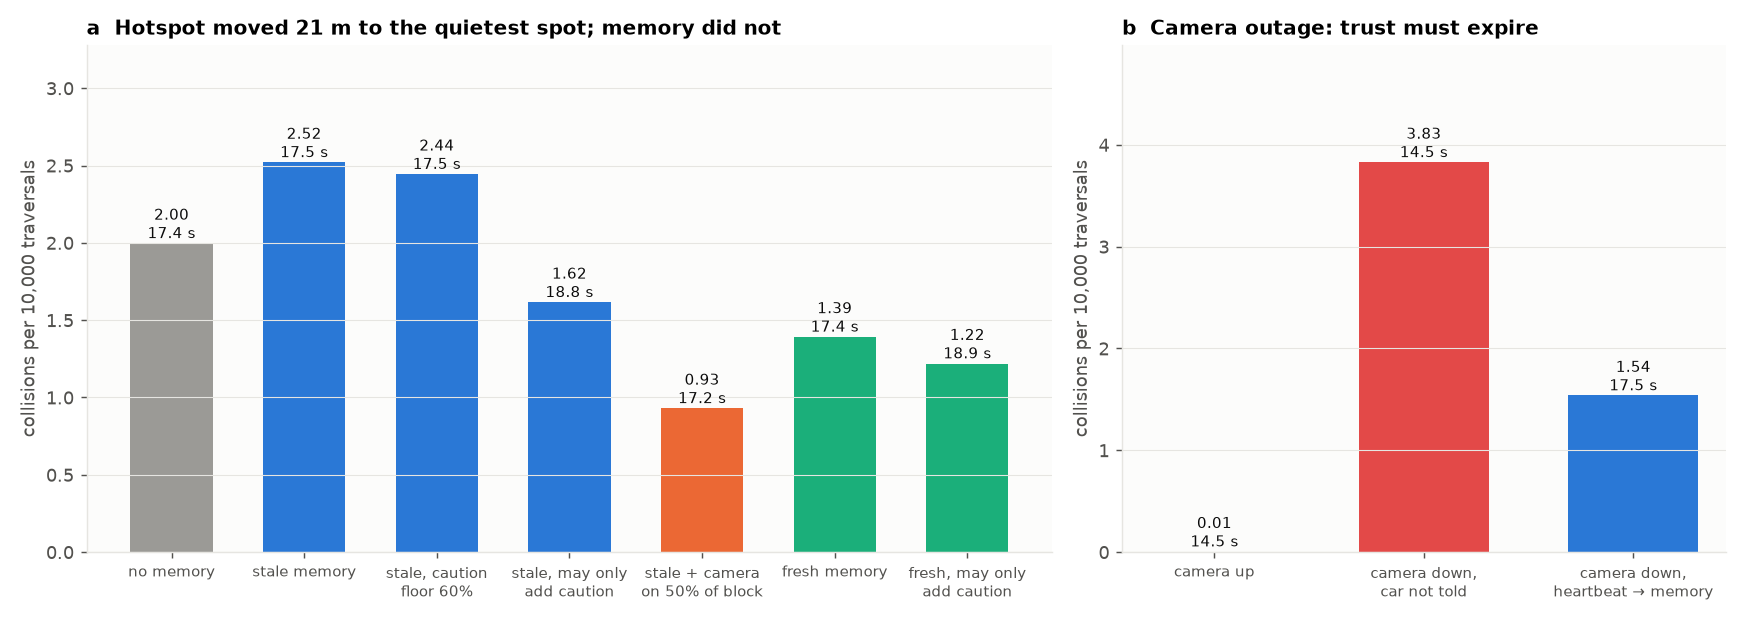
\includegraphics[width=0.95\linewidth]{sim3_robustness.png}
\caption{Collisions per 10{,}000 traversals at the same caution setting. (a) The hotspot moved and memory did not. (b) Camera outage with and without a heartbeat.}
\label{fig:failure}
\end{figure}

\paragraph{Keeping memory fresh.}
The stale-memory failure motivates an update policy. We let the hotspot move while memory keeps receiving observations every 15 minutes and compare four policies: never updating, adding all observations, exponential forgetting (half-life 4\,h), and a sequential change detector.
The detector compares the last hour of observed emergences with the counts memory expects, per 10\,m segment, using the Poisson deviance $G = 2\sum_j [k_j \ln(k_j/\mu_j) - (k_j-\mu_j)]$ against a $\chi^2$ threshold with a per-check level of $10^{-4}$; on detection, memory restarts from the window that triggered it (Figure~\ref{fig:change}).
With a camera the change is noticed after a median of 45 minutes (all of 200 simulated changes within an hour), with 0.3 false alarms per 30 days.
Averaged over the 24 hours after the change, collisions per 10{,}000 traversals are 1.47 with detection, against 2.47 for a memory that is never updated, 1.99 for one that adds all observations (it recovers only after about two days) and 1.65 for forgetting; forgetting, however, costs 8\pct{} more collisions when nothing changes (1.58 versus 1.46), because it always works from little data, while the detector costs nothing.
With a 10\pct{} fleet as the only observer, detection takes a median of 1.25 hours and 10\pct{} of changes go unnoticed within a day; with a 3\pct{} fleet only 19\pct{} are noticed within a day.

\begin{figure}[t]
\centering
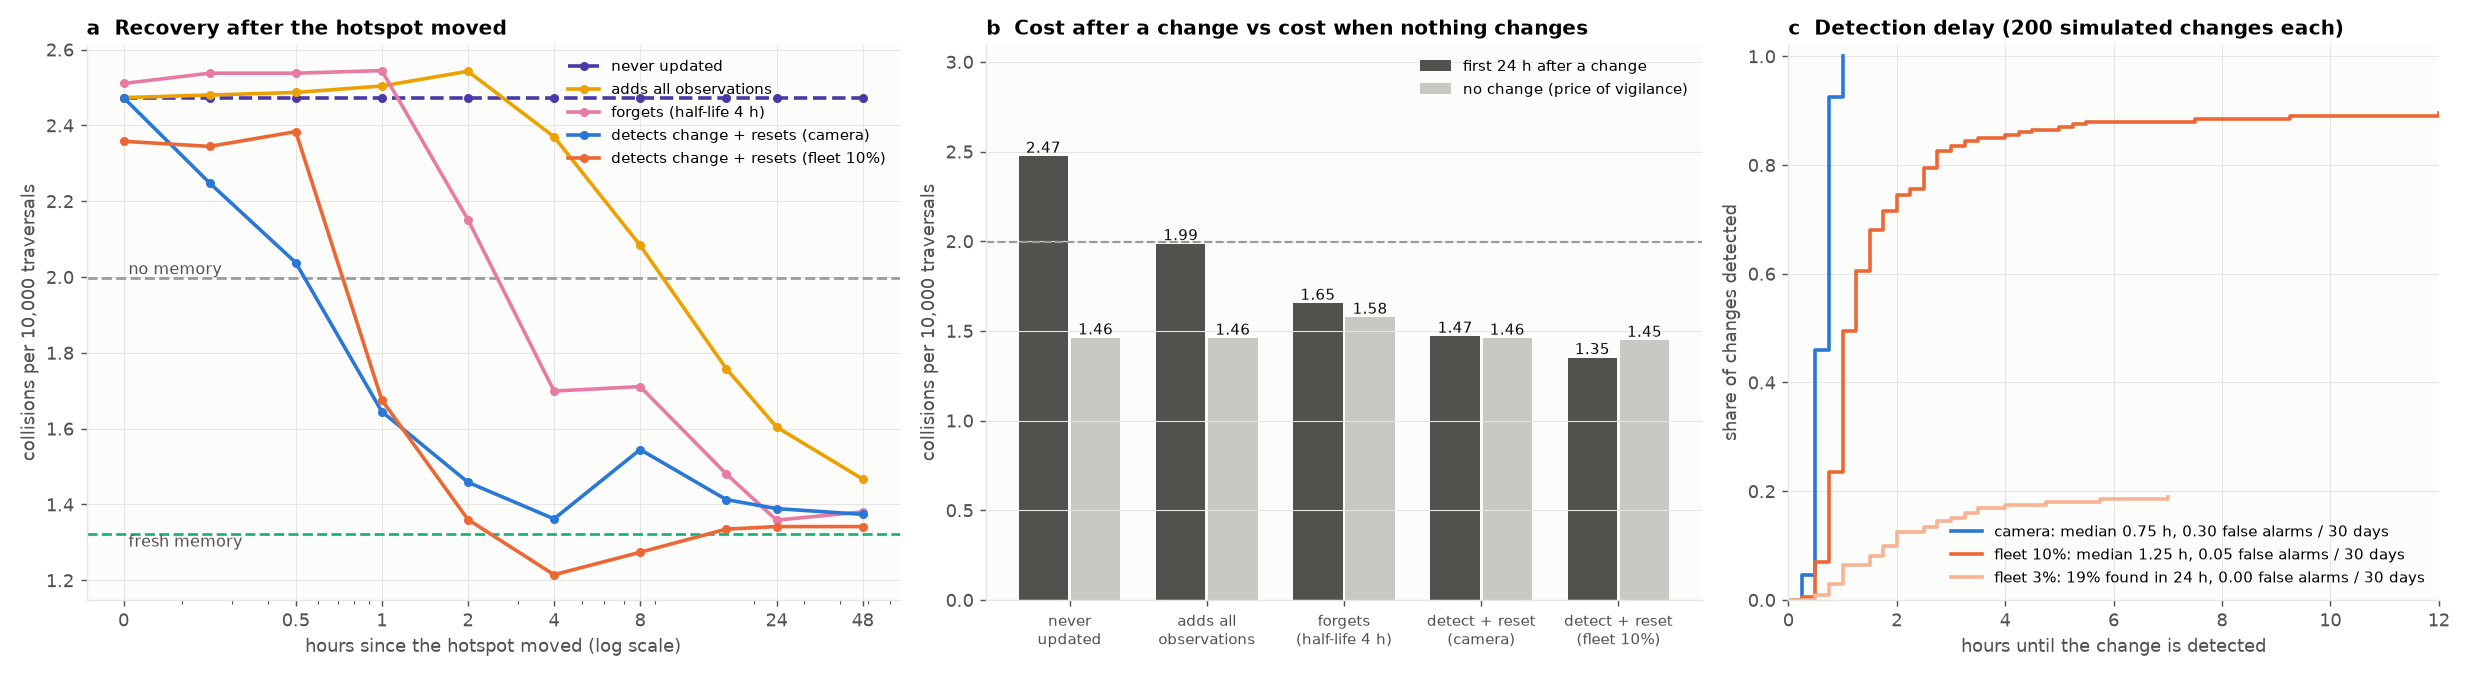
\includegraphics[width=\linewidth]{sim4_change_detection.png}
\caption{Keeping memory fresh after the hotspot moves. (a) Collisions versus hours since the change for four update policies (mean of three observation streams). (b) Mean over the first 24 hours after a change versus the steady-state cost when nothing changes. (c) Detection delay over 200 simulated changes per observer, with false-alarm rates from 40 simulated months without change.}
\label{fig:change}
\end{figure}

\paragraph{Phantoms and silently dropped pedestrians.}
A live camera can also lie: it may report pedestrians who do not exist---benign false positives such as sidewalk walkers taken for crossers, or phantoms injected by an attacker---or silently drop real pedestrians while its heartbeat stays healthy (Figure~\ref{fig:spoof}).
A vehicle that trusts every report brakes hard 1.6 times per phantom and at $\ge 6$\,m/s$^2$ in 28\pct{} of cases; phantoms timed to cross just before the vehicle cause emergency braking in 66\pct{} of cases, and 50 false reports per hour on the block more than triple hard braking (101 to 347 per 1{,}000 traversals).
The defence is \emph{onboard priority}: where the vehicle's own sensor has a clear line of sight to a reported object, only its own perception counts, and a report left unconfirmed for 0.4\,s is discarded; the camera only fills blind spots. This refutes 99\pct{} of phantoms, lowers emergency braking to 0.5\pct{} (1.9\pct{} for timed phantoms, 0\pct{} for phantoms that pop up in view) and costs nothing measurable with an honest camera.
Dropped pedestrians are the dangerous case: with the camera trusted to declare the block clear, collisions rise from 0.005 to 1.04, 2.01 and 3.83 per 10{,}000 traversals when 25, 50 and 100\pct{} of pedestrians are dropped. If the camera may only add caution, the same attack yields 0.43, 0.82 and 1.54---never worse than having no camera---but the vehicle then forgoes the 3\,s the honest camera saves on every block.
The two can be combined by a fleet audit: vehicles report pedestrians they saw in a covered area before the camera had reported them (2.7\pct{} of encounters with an honest camera, 67\pct{} when all are dropped), and a Bernoulli CUSUM on these per-traversal reports, with its threshold set for at most one false revocation per year, revokes trust after a median of 2.5 hours at 10 passes per hour when all pedestrians are dropped and 13 hours when a quarter are.

\begin{figure}[t]
\centering
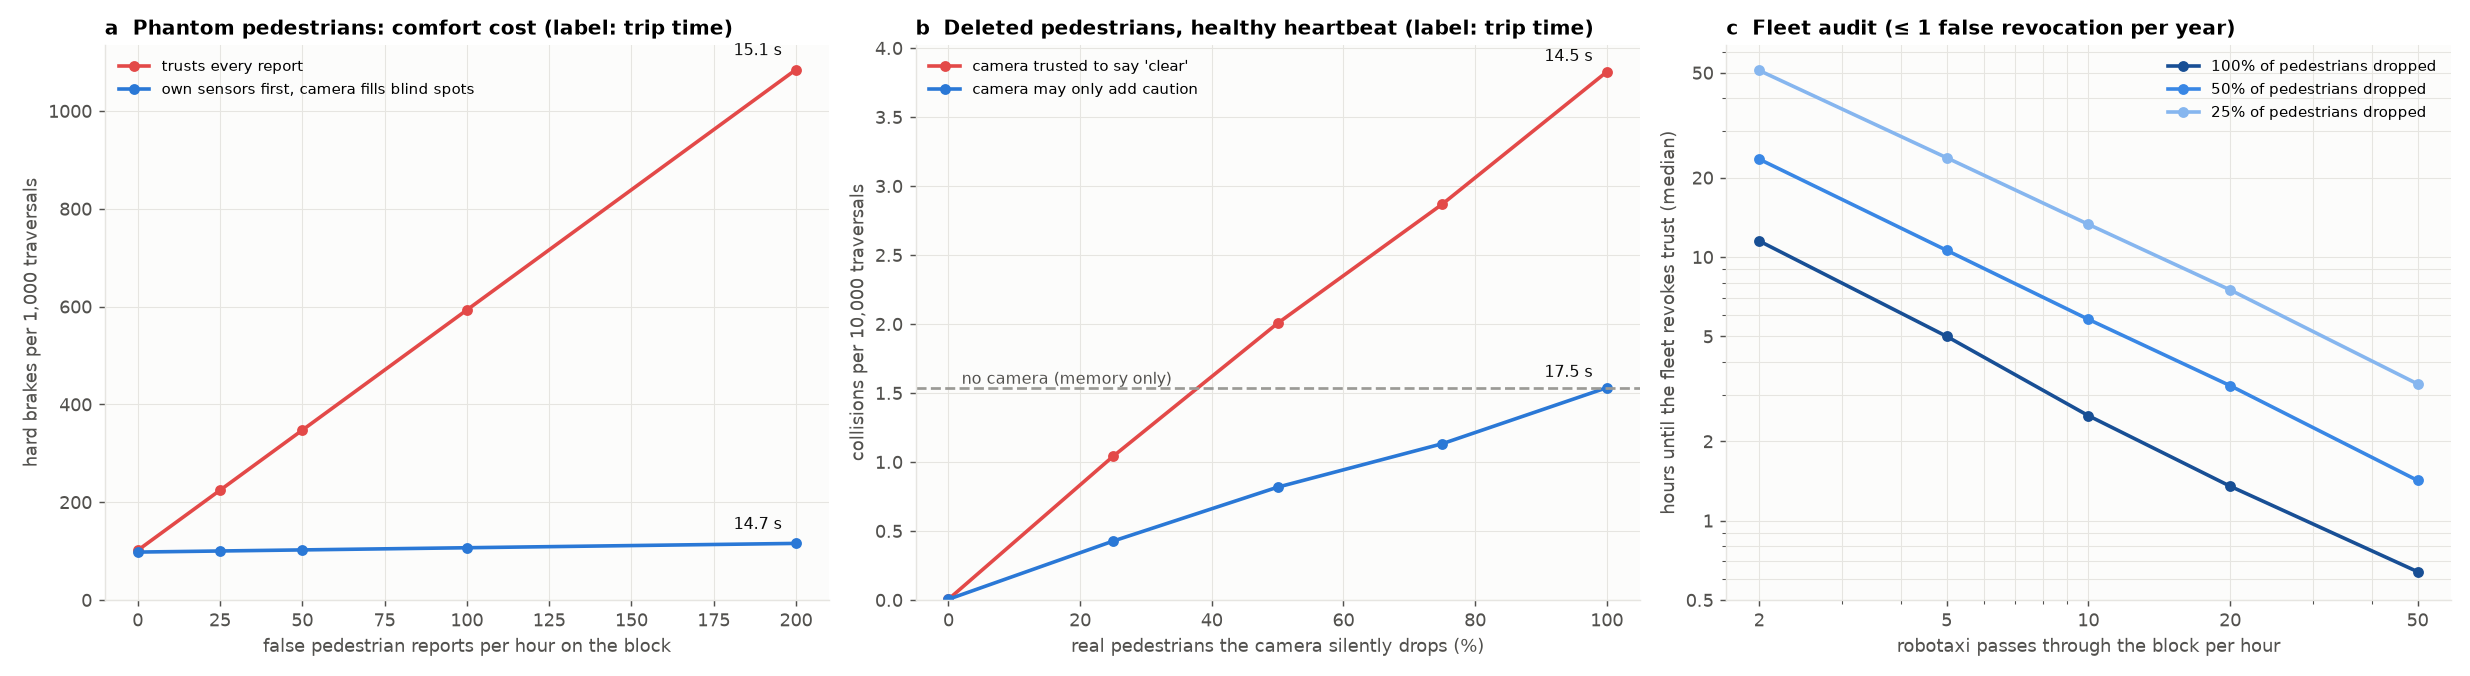
\includegraphics[width=\linewidth]{sim5_spoofing.png}
\caption{A lying camera. (a) Hard braking versus false pedestrian reports per hour, trusting every report versus onboard priority (labels: trip time). (b) Collisions when the camera silently drops a share of real pedestrians, trusted to declare the block clear versus allowed only to add caution. (c) Median time until a fleet audit revokes trust in a dropping camera, with at most one false revocation per year.}
\label{fig:spoof}
\end{figure}



% ============================================================================
\section{Part 3: why fixed cameras, if a fleet can remember?}
\label{sec:fleet}

A fleet memory only knows what passing vehicles happened to see, and records a pedestrian where and when a vehicle first saw it.
We treat each of the 4{,}828 driving vehicles in TGSIM as a potential fleet car with a 50\,m roof sensor whose 2-D line of sight can be blocked by other vehicles; a random share of them (the penetration) is equipped.
The fleet memory is built from equipped vehicles' first sightings in the first 79 minutes and scored on the same held-out window as the camera memory.
In the simulator, the share of time each metre of kerb is watched by equipped vehicles---measured on the real traffic of the block, 184 driving vehicles per hour---thins the observations from which memory is estimated.

\begin{table}[t]
\centering\small
\caption{Fleet versus infrastructure memory on the same real traffic. Time to full benefit: simulator, two memory draws per setting (indicative).}
\label{tab:fleet}
\begin{tabularx}{\linewidth}{Xccc}
\toprule
Memory source (equipped vehicles / h) & Pedestrians seen & Gain: all / off-crosswalk & Time to full benefit \\
\midrule
Fixed cameras & 100\pct & 2.27 / 0.84 bits & $\approx$\,1\,h \\
Fleet, 100\pct{} (184/h) & 98\pct & 2.24 / 0.81 bits & $\approx$\,1\,h \\
Fleet, 30\pct{} ($\approx$\,55/h) & 71\pct & 2.14 / 0.71 bits & --- \\
Fleet, 10\pct{} ($\approx$\,18/h) & 37\pct & 1.96 / 0.62 bits & $\approx$\,4\,h \\
Fleet, 3\pct{} ($\approx$\,5/h) & 17\pct & 1.62 / 0.37 bits & $\approx$\,16\,h \\
\bottomrule
\end{tabularx}
\end{table}

\begin{figure}[t]
\centering
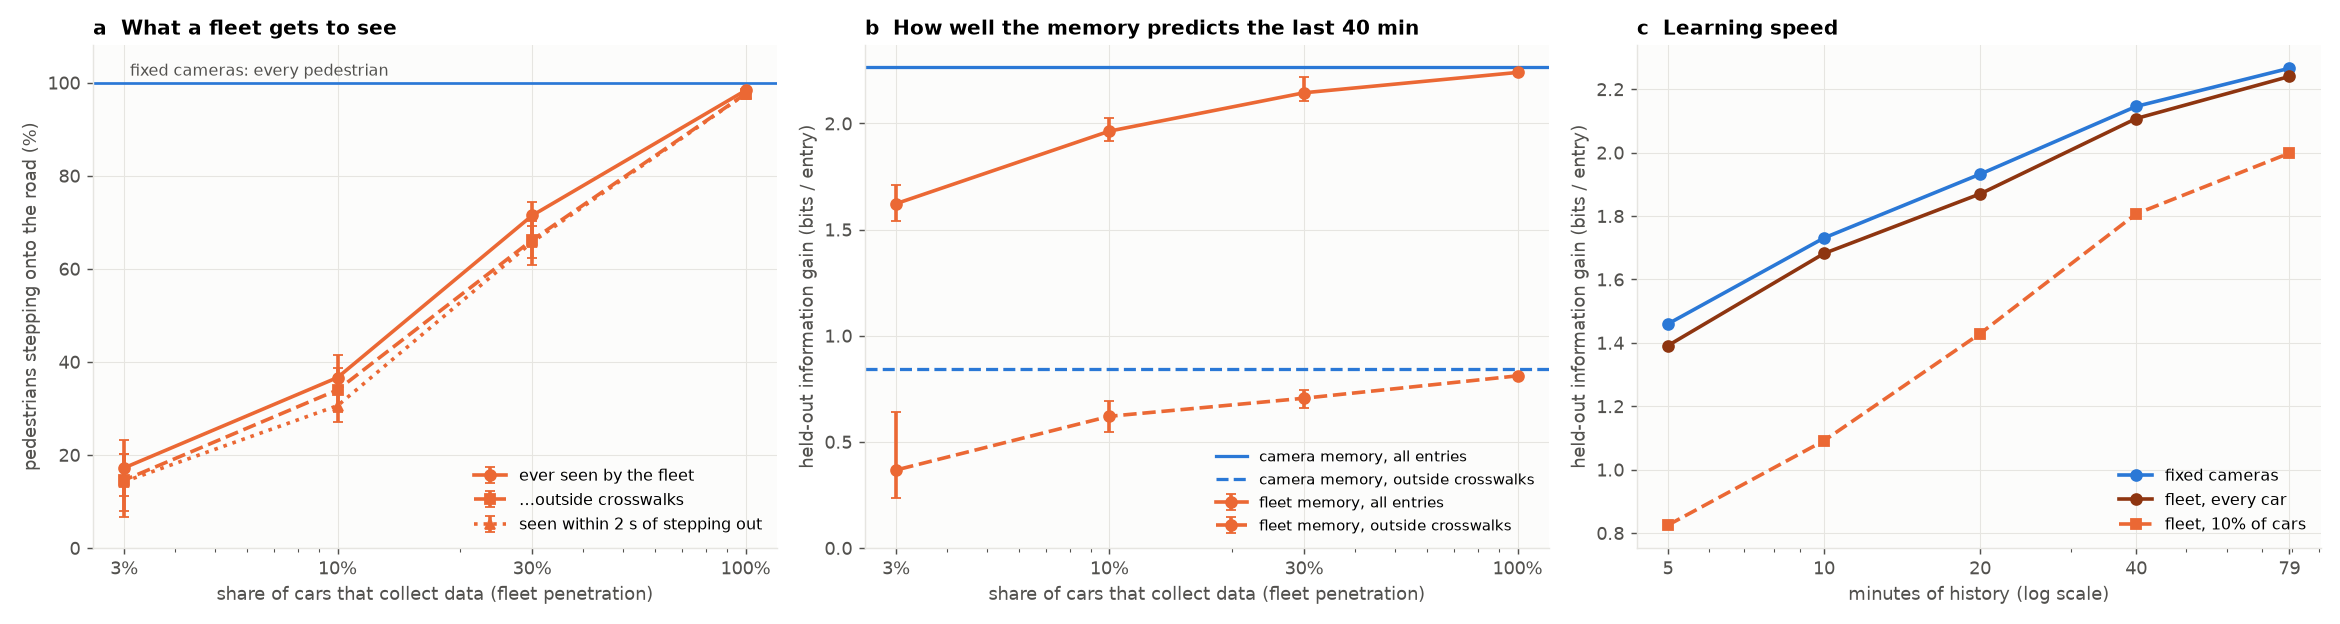
\includegraphics[width=\linewidth]{fleet1_real_data.png}
\caption{Fleet memory on real traffic: (a) share of pedestrians seen, (b) held-out information gain versus penetration, (c) learning speed of camera and fleet memory.}
\label{fig:fleet}
\end{figure}

When a car is present it sees the pedestrian almost as well as a camera: median 0.2\,s late and 0.2\,m from the true entry point (Table~\ref{tab:fleet}, Figure~\ref{fig:fleet}).
What limits a fleet is exposure---equipped vehicles per hour times hours.
A 10\pct{} fleet's memory after 79 minutes (1.96 bits) matches the camera memory after roughly 30 minutes, and in the simulator it needs about 4 hours to deliver the full planning benefit that a camera delivers in about one; a 3\pct{} fleet needs about 16 hours and, after one hour, is worse than no memory.
Entries outside crosswalks, where hidden-pedestrian risk lives, are where the fleet lags most.
Correcting for per-location exposure made no difference here because equipped vehicles watched the kerb fairly uniformly (19--36\pct{} of the time at 10\pct), but it matters where coverage is uneven.
This rush-hour block is the fleet's best case; the fleet is idealised (perfect detection within 50\,m, every sighting uploaded) and can only observe pedestrians the cameras also tracked, so the fleet numbers are upper bounds.

% ============================================================================
\section{Part 4: memory and live signals at an instrumented intersection}
\label{sec:dlr}

Part~1 left an open end: most of the error in predicting vehicles was longitudinal stop-and-go at signals, which a memory of the place cannot know.
The DLR Urban Traffic dataset \citep{dlr_ut} closes it. Fourteen infrastructure multi-sensor systems around a signalised research intersection in Braunschweig recorded one full day (Sunday 24 September 2023, 00:00--24:00 UTC) at 20\,Hz, together with the states of all 30 traffic lights at 1\,Hz; after downsampling to 10\,Hz the day contains 28{,}378 vehicles, 3{,}153 cyclists and 765 pedestrians.
We predict a vehicle's speed class 3\,s ahead (stopped, crawling, slow, moving) from four sources: area-wide statistics; the live phase of the governing light alone; location memory alone (per 4\,m cell and heading); and memory plus live phase. Which light governs a place is learned from memory as the light whose green state carries most mutual information about vehicles there being stopped 3\,s later; 244 of 1{,}035 places acquire a governing light (Figure~\ref{fig:dlr}a). Memory is built from even hours and tested on odd hours, so both cover day and night; intervals resample whole vehicles.

\begin{figure}[t]
\centering
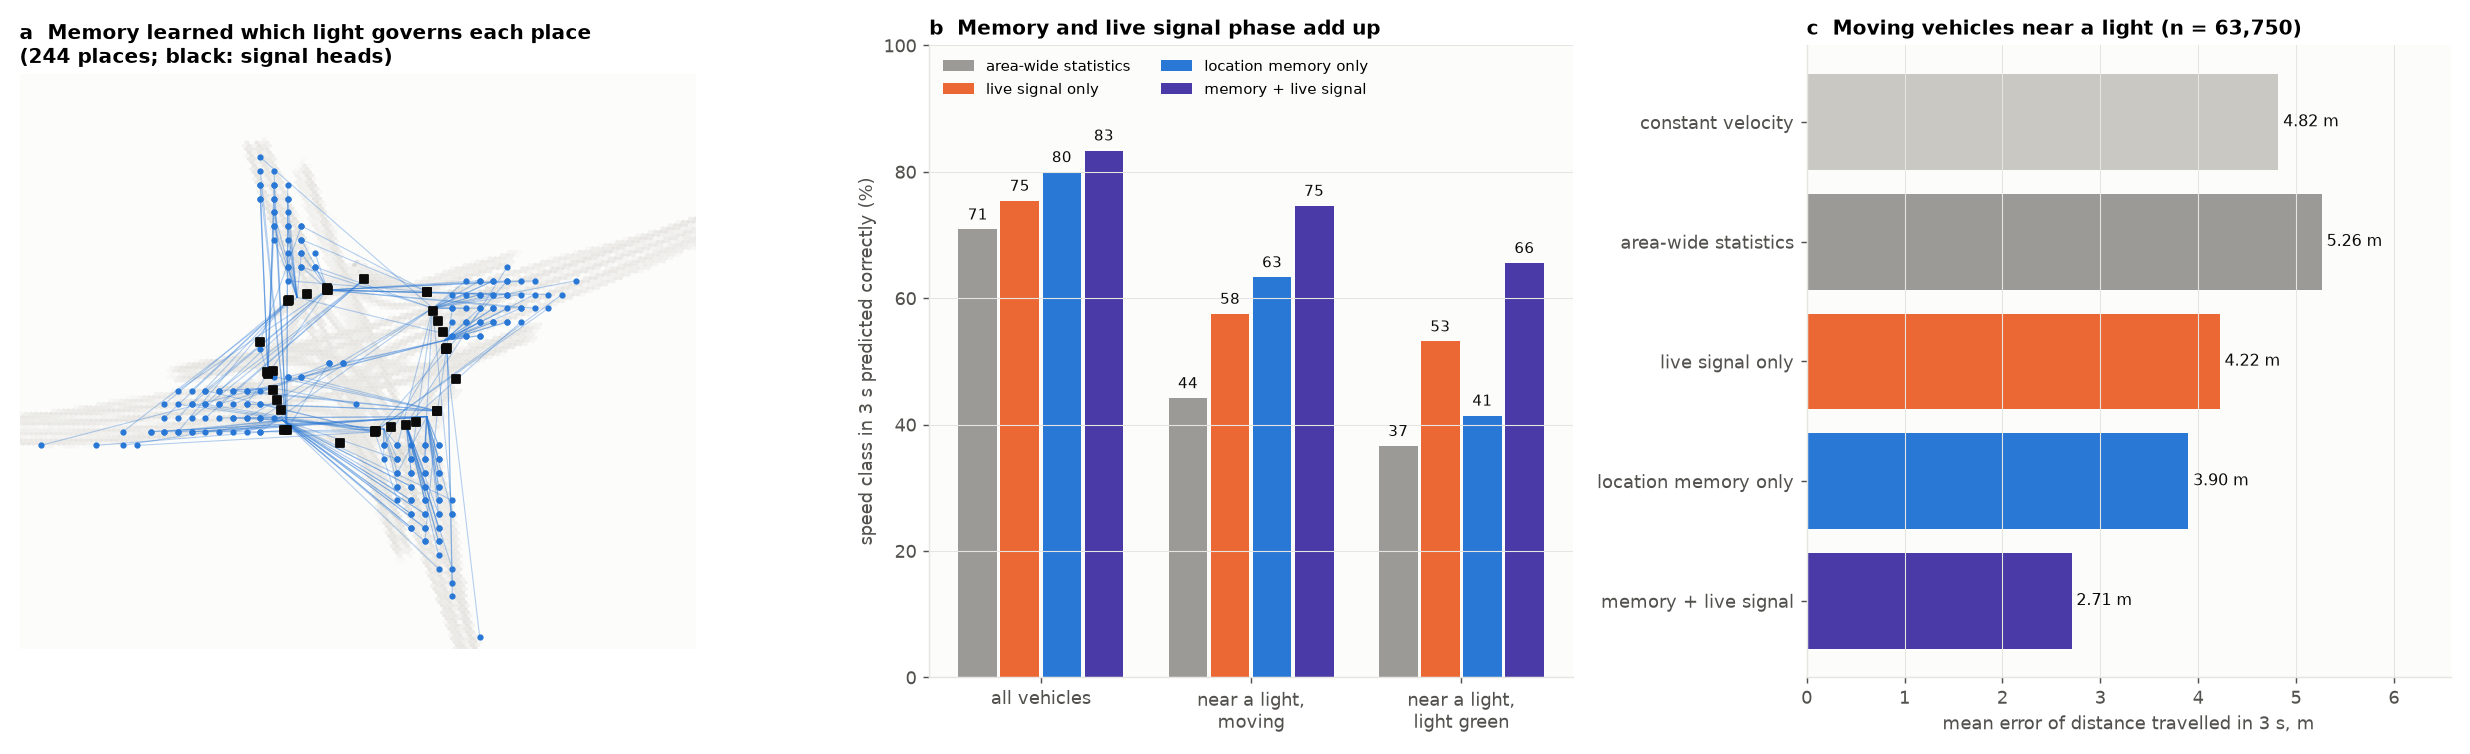
\includegraphics[width=\linewidth]{dlr1_signal_memory.png}
\caption{A full day at the DLR research intersection. (a) Places (blue) linked to the traffic light that memory learned governs them (black squares: signal heads). (b) Speed class 3\,s ahead predicted correctly by each source. (c) Error of the distance a moving vehicle near a light travels in 3\,s.}
\label{fig:dlr}
\end{figure}

The two sources add up (Figure~\ref{fig:dlr}b,c). For moving vehicles near a governing light (63{,}750 test samples) the speed class is predicted correctly 44\pct{} of the time from area-wide statistics, 58\pct{} from the live phase alone, 63\pct{} from memory alone and 75\pct{} from both (information gain 0.27, 0.53 and 0.82 bits per sample); the error of the distance travelled in 3\,s falls from 4.82\,m under constant velocity to 4.22\,m with the live phase, 3.90\,m with memory and 2.71\,m with both ($-44\pct$). When the light is green, the live phase alone gains 0.73 bits and memory adds another 0.40.
Conditioning memory additionally on day versus night does not help (0.27 versus 0.26 bits by day, 0.26 versus 0.25 at night): once the current speed and the light are known, the place behaves alike at any hour, and splitting the data only thins it.
Vehicle--VRU conflicts remain rare even over a full day: 24 with TTC $\le 1.5$\,s (22 with cyclists), clustered at two crossing points; the 8 conflicts of even hours already locate 15 of the 16 of odd hours within the top 10\pct{} of road area, but samples this small only indicate that conflict hot spots are stable.

% ============================================================================
\section{Part 5: does memory transfer across days?}
\label{sec:pneuma}

All earlier memories were built and tested within a single day. pNEUMA \citep{barmpounakis2020pneuma,pneuma_zenodo} recorded downtown Athens with a swarm of drones on four weekday mornings (Wednesday 24, Monday 29, Tuesday 30 October and Thursday 1 November 2018). We use two drone areas and the same four half-hours (08:30--10:30) of every morning, streamed from the published archive with range requests and downsampled to 5\,Hz: 74{,}405 vehicles (28{,}163 cars, 26{,}807 motorcycles, 14{,}213 taxis and others), vehicles only.
For each test half-hour we build memory (per 4\,m cell and heading, as in Part~4) from the other half-hours of the same morning (1.5\,h), from the \emph{same half-hour on the other three mornings} (also 1.5\,h), from all half-hours of the other mornings (6\,h), or from everything else (7.5\,h), and score it against area-wide statistics on the heading and the speed class 3\,s ahead (Figure~\ref{fig:pneuma}).

\begin{figure}[t]
\centering
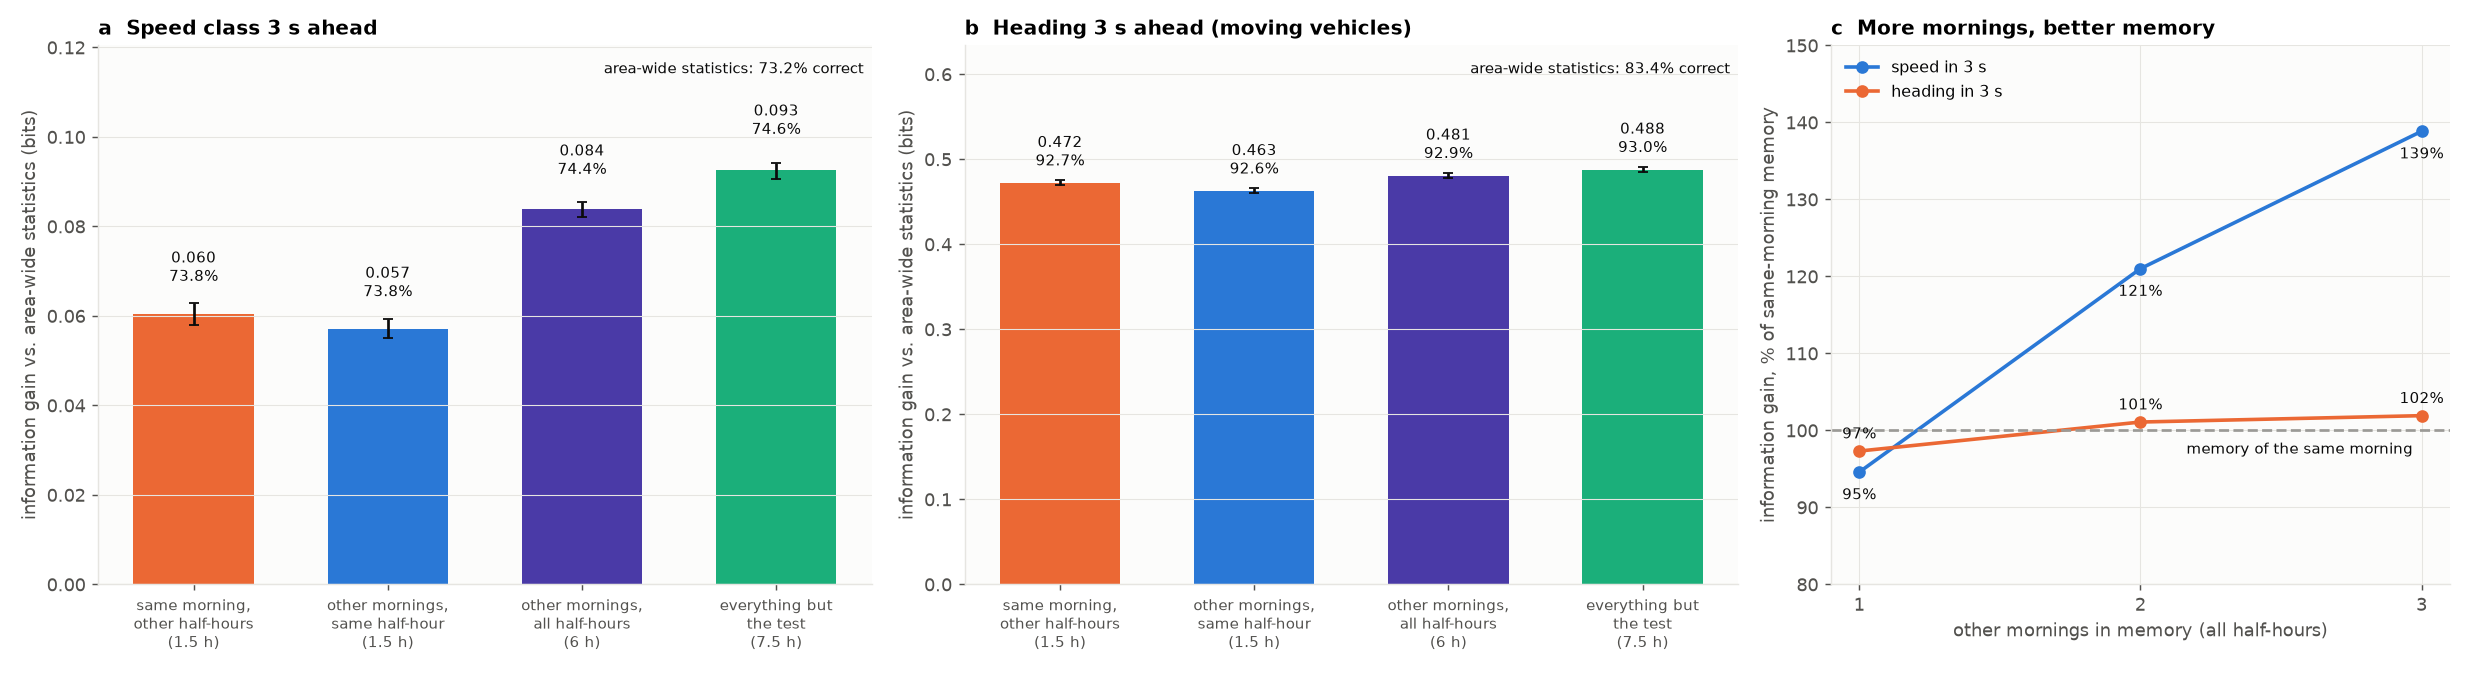
\includegraphics[width=\linewidth]{pneuma1_cross_day.png}
\caption{Cross-day transfer on four weekday mornings in Athens. Information gain over area-wide statistics (labels: share predicted correctly) for (a) the speed class and (b) the heading 3\,s ahead, by where memory comes from. (c) Gain of memory from one to three other mornings, relative to memory of the same morning.}
\label{fig:pneuma}
\end{figure}

Memory transfers across days. For the heading of moving vehicles, area-wide statistics are right 83.4\pct{} of the time; memory of the same morning 92.7\pct{} (0.472 bits per sample) and memory of the other mornings, at equal volume, 92.6\pct{} (0.463 bits): 98\pct{} of the information. For the speed class the figures are 0.060 and 0.057 bits (94\pct). More mornings help: memory from all half-hours of three other mornings exceeds same-morning memory (102\pct{} for heading, 139\pct{} for speed).
Without the signal phase, however, memory predicts speed in dense Athens traffic only weakly (the 3\,s distance error falls from 1.98 to 1.89\,m), which is consistent with Part~4: speed needs memory \emph{and} live signal data. Cross-day transfer for pedestrians is tested in Part~7 (\S\ref{sec:ind}).

% ============================================================================
\section{Part 6: where does infrastructure pay off?}
\label{sec:econ}

The previous parts measure benefits in bits, collisions and seconds. A city deciding where to put cameras needs them in money, against costs.
The unit of analysis is one block face like the simulated street: 90\,m of kerb with parked cars. The baseline is what a fleet can do alone: robotaxis already use a fleet-learned memory (Part~3), fresh wherever they pass often enough. Against it we value four options: location memory from \emph{existing} city cameras (software only); \emph{new} cameras for memory; a \emph{live} camera with a roadside unit whose ``clear'' the vehicle trusts, protected by the heartbeat, onboard priority and fleet audit of E9; and the same hardware used so that the vehicle is \emph{never worse} than without it, i.e.\ at its old speed, with the benefit taken as safety only.

\paragraph{What one traversal gains (E14).}
For each concentration of pedestrian activity of E6, the simulator compares the risk--time curve of each source with the no-memory planner at the operating point: seconds saved at equal risk and collision reduction at equal time. On this street memory saves 1.2\,s per traversal (0.2--1.7\,s from a uniform to a strongly concentrated street); a trusted live camera saves about 3.45\,s at any unevenness, because the speed limit binds. A camera whose reports may only add caution saves 1.2--3.4\,s only if the operator raises its overall speed, which gives up the guarantee of never being worse than without the camera.

\paragraph{Valuation.}
Seconds are valued at the USDOT value of travel time, \$21.10 per person-hour \citep{usdot_bca2025}, times 0.7 riders per traversal, plus \$10 per vehicle-hour for the operator, and only on the half of traversals where pedestrian risk, not traffic ahead or a signal, limits the vehicle's speed: \$0.0034 per second saved. Avoided crashes are valued with the USDOT crash costs (\$13.2\,M per fatality, \$229{,}800 per injury of unknown severity; 3\pct{} fatal, against 9.7\pct{} of injured or killed pedestrians nationally \citep{nhtsa_ped2023}) at the robotaxi pedestrian-injury crash rate of 7 in 271.3\,M rider-only miles \citep{waymo_hub}, times three for a busy block and 0.3 for the share of crashes of the occluded step-out type. Costs are two cameras at the median furnished-and-installed price of \$6{,}220 \citep{itsjpo_costs}, \$10{,}000 of site works, a roadside unit at \$11{,}000 \citep{itsa_v2x2023} and \$5{,}000 of edge computing for the live options, 10\pct{} of capital a year for maintenance and \$600 per camera-year for analytics; the camera memory beyond fleet memory follows from the staleness after a change (E8: about 0.8\,h for a camera or a fleet passing 18 times an hour, 14\,h at 5.5 passes per hour) at four changes a year. Benefits and costs are discounted at 7\pct{} over ten years. Parameters without a published source are assumptions with stated ranges; a Monte Carlo draws all of them from triangular distributions.

\begin{figure}[t]
\centering
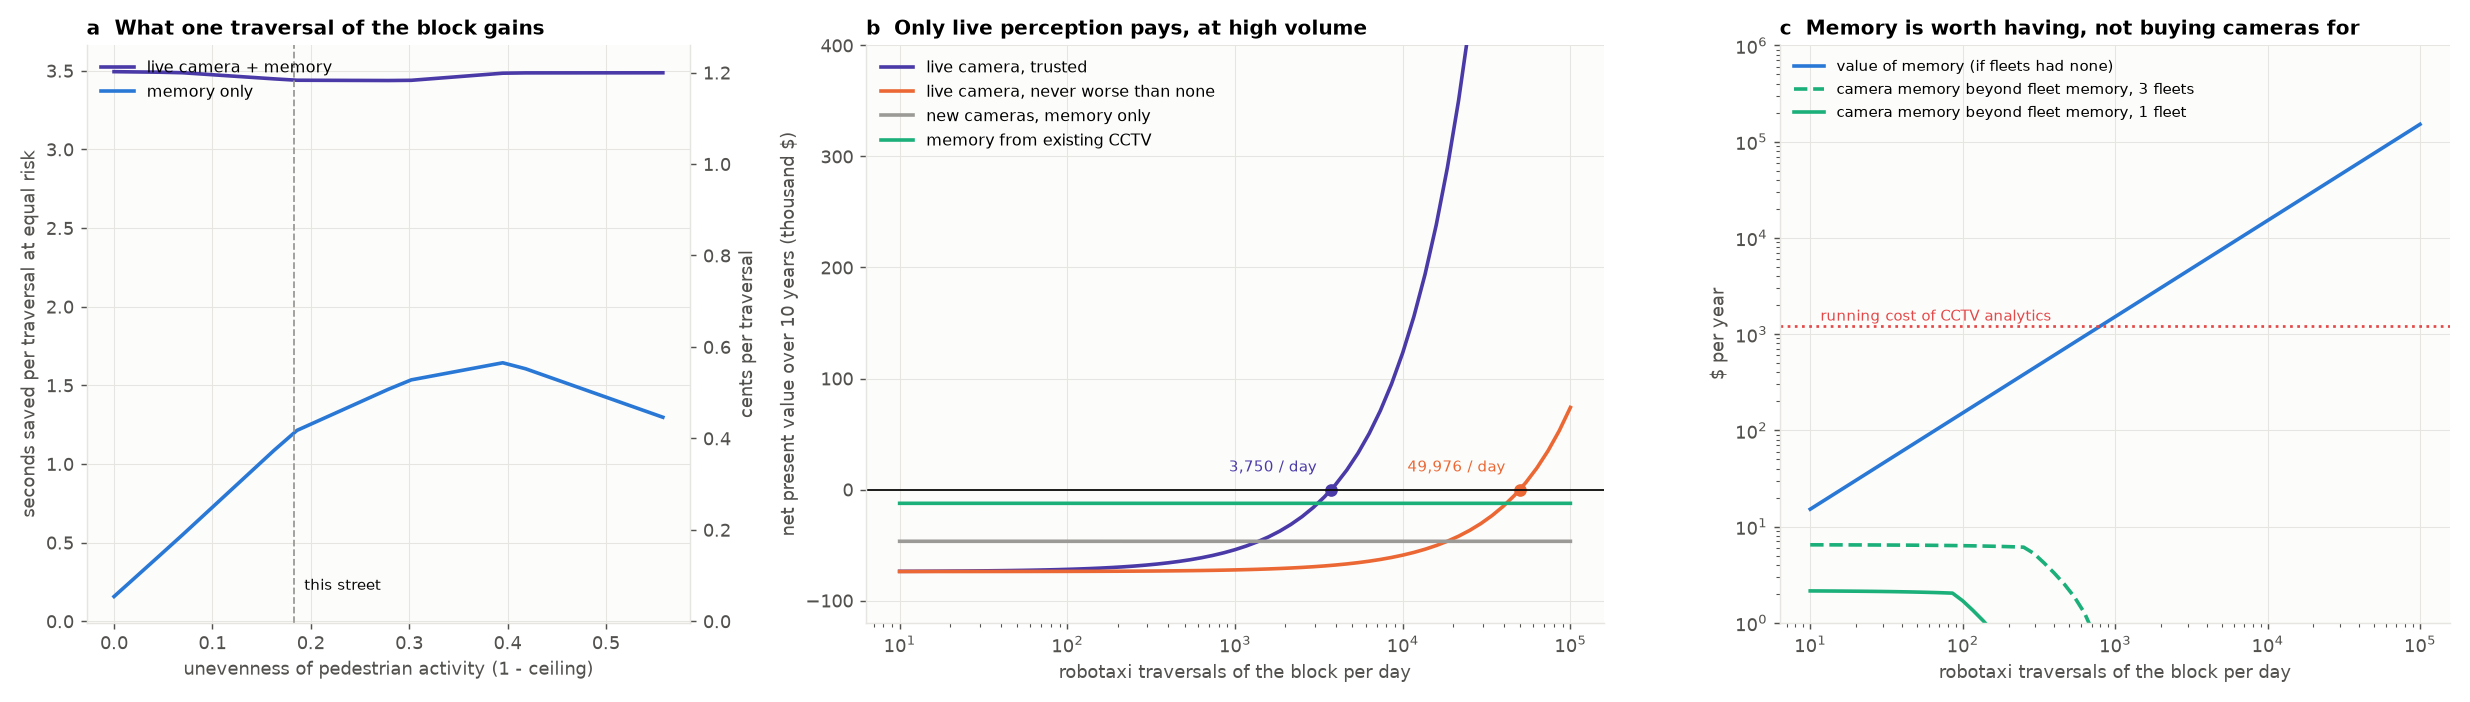
\includegraphics[width=\linewidth]{econ1_value.png}
\caption{Cost-benefit per block face. (a) Seconds saved per traversal at equal risk and their value, by unevenness of pedestrian activity. (b) Net present value over ten years by option at this street's unevenness, with break-even volumes. (c) Annual value of memory if fleets had none, the value camera memory adds to fleet memory with one or three fleets that do not share data, and the running cost of analytics on existing cameras.}
\label{fig:econ}
\end{figure}

\begin{table}[t]
\centering
\small
\caption{Cost-benefit per block face at this street's unevenness (2023 dollars, 7\pct, 10 years).}
\label{tab:econ}
\begin{tabular}{@{}lrrr@{}}
\toprule
Option & Value & Cost & Break-even \\
 & & & (traversals/day) \\
\midrule
Live camera, trusted & 2.23\,s (0.77\,\textcent) per traversal & \$38{,}440 + \$5{,}044/yr & 3{,}750 \\
Live camera, never worse & 0.06\,\textcent{} per traversal (safety) & same & $\approx$\,50{,}000 \\
Memory from existing CCTV & $\le$\,\$6.5/yr beyond fleet memory & \$1{,}770/yr & never \\
New cameras, memory only & same & \$22{,}440 + \$3{,}444/yr & never \\
\bottomrule
\end{tabular}
\end{table}

\paragraph{Results.}
Live perception is what cameras sell, and it pays at high robotaxi volume (Table~\ref{tab:econ}, Figure~\ref{fig:econ}): a trusted live camera breaks even at 3{,}750 traversals a day (90\pct{} interval 2{,}340--7{,}450 over parameter uncertainty; 3{,}410 at a 3.1\pct{} discount rate), about a third of a street carrying 10{,}000 vehicles a day. The probability of a positive net present value is 19\pct{} at 3{,}000 traversals a day and 98\pct{} at 10{,}000. The break-even hardly depends on the unevenness of pedestrian activity, since the live camera's gain is capped by the speed limit; it is moved most by the share of traversals where traffic ahead does not bind, the value of a vehicle-hour and the cost of the roadside unit (Figure~\ref{fig:econ_decision}).
The benefit is time, not avoided crashes: robotaxis already hit pedestrians rarely, so memory taken as safety is worth 0.023\,\textcent{} per traversal against 0.41\,\textcent{} taken as time; at the human benchmark crash rate the two would be comparable. The cheapest guarantee, never being worse than without the camera, therefore costs almost the whole business case, which is the economic argument for the trust machinery of E9.
Memory is worth having but not worth buying cameras for: once a fleet passes about 18 times an hour it recovers from a change as fast as a camera, so camera memory adds at most a few dollars a year per site to fleet memory, even with three fleets that do not share data. Existing cameras would pay for memory alone only for an operator without its own memory (from about 1{,}170 traversals a day).
A per-traversal fee that covers a live camera is 0.96\,\textcent{} at 3{,}000 traversals a day and 0.29\,\textcent{} at 10{,}000, against a value of 0.77\,\textcent{} to the operator: on busy corridors a city could sell the live feed.

\begin{figure}[t]
\centering
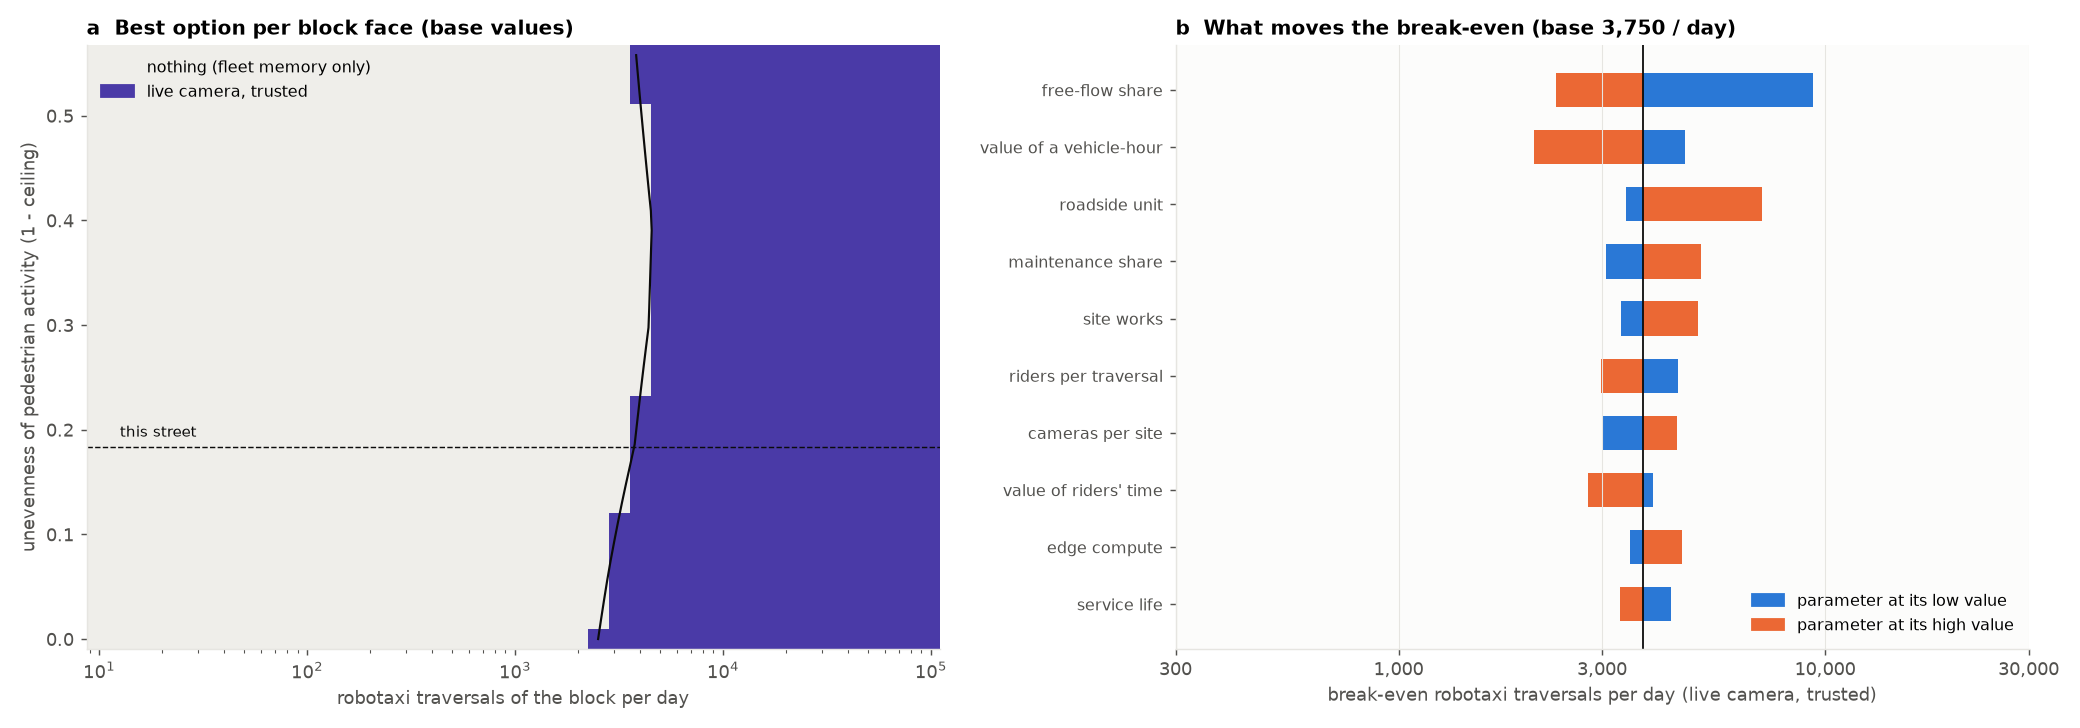
\includegraphics[width=\linewidth]{econ2_decision.png}
\caption{(a) Option with the highest net present value per block face, by robotaxi volume and unevenness of pedestrian activity (base values; line: break-even of the trusted live camera). (b) Break-even volume of the trusted live camera when one parameter at a time is set to the low or high end of its range.}
\label{fig:econ_decision}
\end{figure}

% ============================================================================
\section{Part 7: do pedestrians cross at the same places on other days?}
\label{sec:ind}

Part~5 had no pedestrians. The inD dataset \citep{bock2020ind} recorded four intersections in Aachen from a drone, 33 recordings of 13--22 minutes with all road users in one metric frame per site. We group recordings into sessions---consecutive recordings on the same weekday---which leaves three sites with several sessions: site~1 (Tuesday, Monday, a second Tuesday session; 3.1\,h), site~2 (Tuesday, Wednesday; 4.0\,h) and site~4 (Wednesday, Tuesday, Monday; 1.8\,h).
The roadway of a site is where vehicles drive, taken from all sessions because it is geometry rather than behaviour; a road entry is a pedestrian stepping onto it after at least a second off it. For each recording, memory of road entries (a 1\,m grid smoothed with $\sigma=1.5$\,m, mixed with 10\pct{} uniform) is built from the other recordings of the same session, from other sessions subsampled to the same number of entries (20 draws), or from all other sessions, and scored on the recording's own entries against a uniform prior over the roadway, with intervals that resample whole pedestrians.

\begin{figure}[t]
\centering
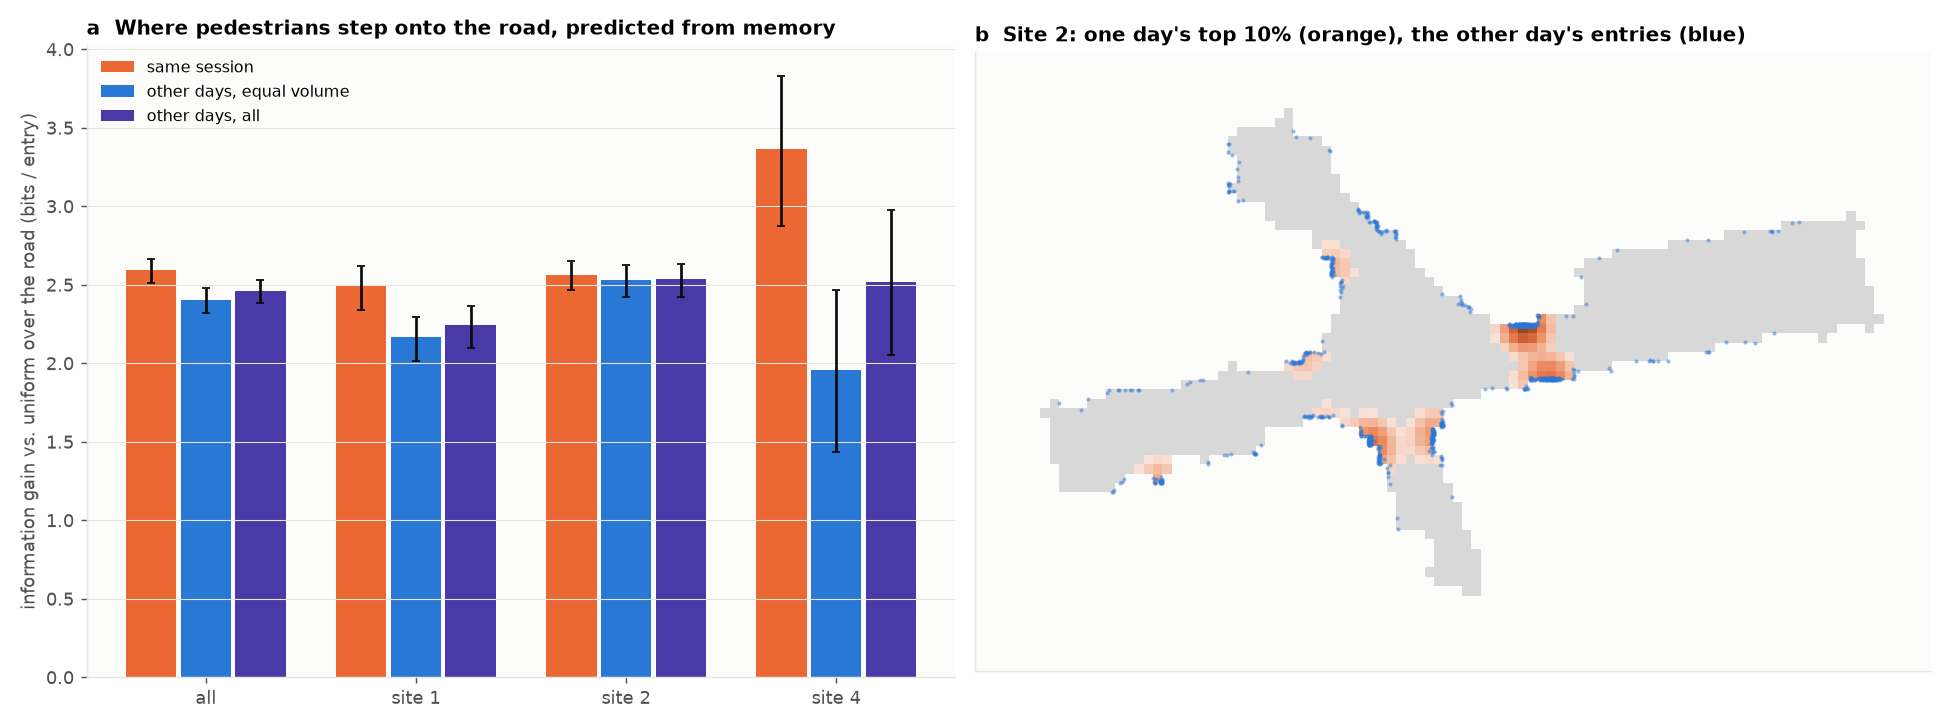
\includegraphics[width=\linewidth]{ind1_cross_day.png}
\caption{Pedestrian memory across days at four intersections in Aachen (inD). (a) Information gain per held-out road entry over a uniform prior on the roadway, by where memory comes from. (b) Site~2: the 10\pct{} of road area ranked highest by memory from one day and the road entries of the other day.}
\label{fig:ind}
\end{figure}

Pedestrian memory transfers across days (Figure~\ref{fig:ind}). Over 2{,}542 held-out entries, same-session memory gains 2.59 bits per entry [2.51, 2.66], memory from other days at equal volume 2.40 [2.32, 2.48]---93\pct{} of the information---and all other days 2.46 [2.38, 2.53]; 78\pct{} of a recording's entries fall into the 10\pct{} of road area that memory from other days ranks highest (79\pct{} for same-day memory). The ratio is 99\pct{} at the busiest site (1{,}718 entries), 87\pct{} at site~1 and 58\pct{} at site~4, where equal volume leaves only about 47 entries of memory and the interval is wide.

% ============================================================================
\section{Part 8: does memory make pedestrian forecasts better on other days?}
\label{sec:ind_pred}

Predicting road entries is a statistic of a place; a planner needs forecasts of individual road users. On the three inD sites with several sessions we take every pedestrian or cyclist in motion every 0.4\,s (263{,}627 anchors, 5{,}215 tracks, 22\pct{} cyclists) and predict its position 1, 2 and 3\,s ahead from the last 1.2\,s of its track. Four predictors: constant velocity; memory alone, the mean displacement of road users who were in the same 1\,m cell heading the same way; gradient boosting on the agent's own recent motion (positions 0.4, 0.8 and 1.2\,s back in its own frame, speed, change of speed, class), predicting the residual to constant velocity; and the same model with memory features at 1\,m and 3\,m resolution. Evaluation is leave-one-session-out, so the test session is a day the model has not seen; memory comes only from other days, also for training rows, whose memory excludes their own session, so that the model never learns to trust a memory containing its own future.

\begin{figure}[t]
\centering
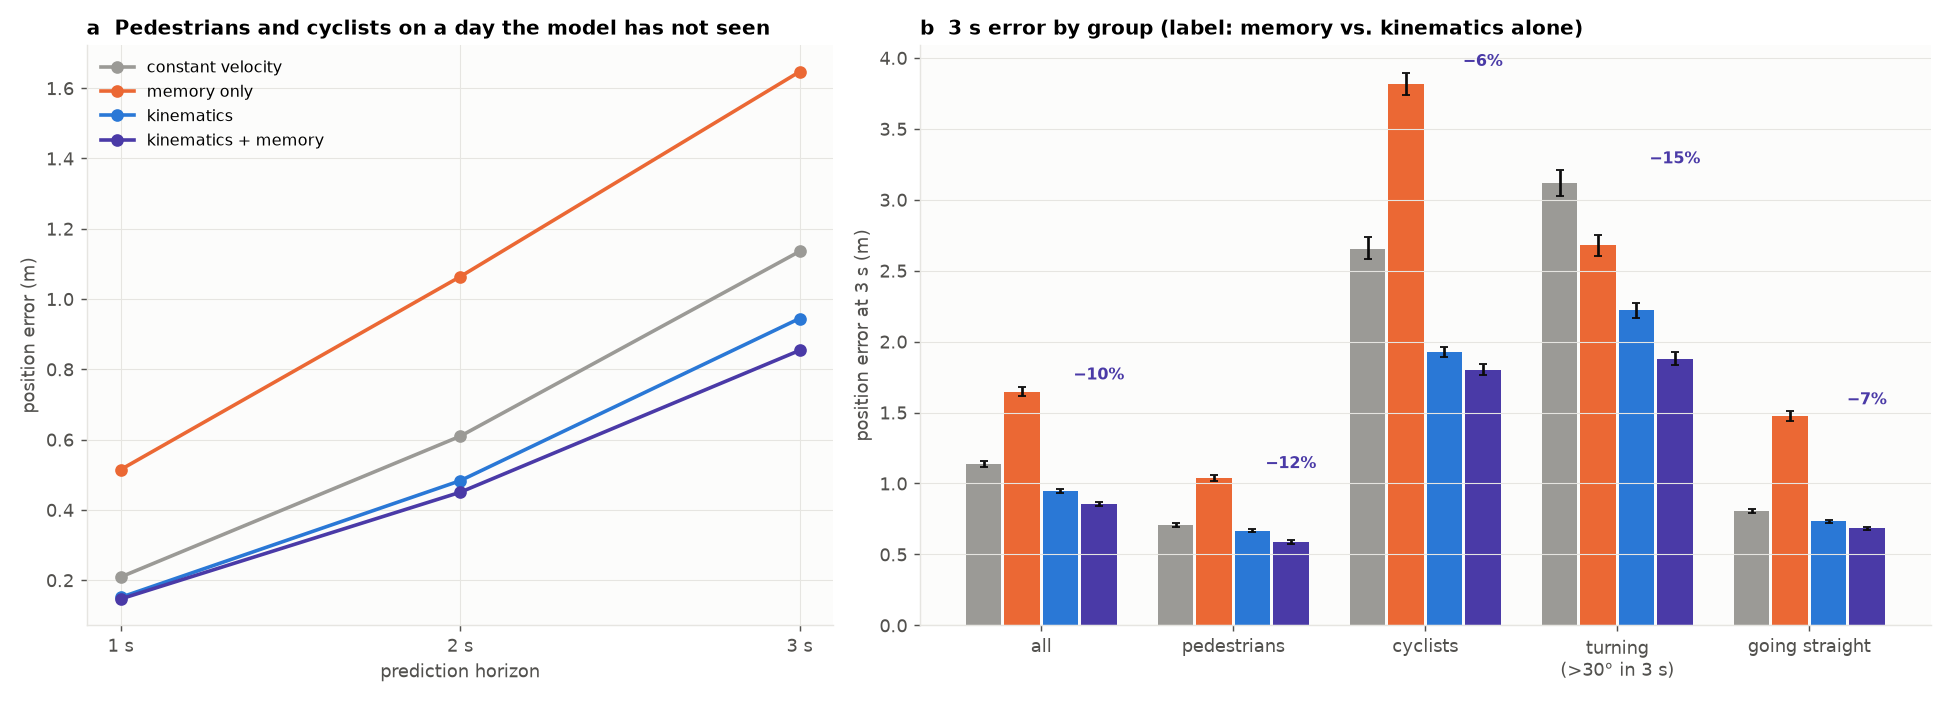
\includegraphics[width=\linewidth]{ind2_prediction.png}
\caption{Forecasts of pedestrians and cyclists on a day the model has not seen (inD, leave-one-session-out). (a) Position error by horizon. (b) Error at 3\,s by group, with 95\pct{} intervals resampling whole tracks; labels give the change from adding memory to the kinematic model.}
\label{fig:ind_pred}
\end{figure}

Memory from other days improves the forecast in each of the eight held-out sessions (Figure~\ref{fig:ind_pred}). The 3\,s error falls from 1.14\,m (constant velocity) and 0.94\,m (kinematics) to 0.85\,m with memory, a paired difference of $-0.091$\,m [$-0.095$, $-0.087$]; by 12\pct{} for pedestrians, 6.5\pct{} for cyclists and 15\pct{} ($-0.34$\,m) for the 14\pct{} of anchors that turn by more than 30$^\circ$ within 3\,s---the lateral manoeuvres that current predictors miss in dense mixed traffic \citep{chen2026hetrod}. Memory alone is worse than constant velocity (1.65\,m): it knows where people go but not how fast this one walks, so it is an addition to a motion model, not a replacement.

% ============================================================================
\section{Discussion}
\label{sec:discussion}

\paragraph{Design rules.}
Five rules follow from the experiments.
(1)~\emph{A prior, not an oracle}: the vehicle decides; the city informs, with an age and a confidence on every message.
(2)~\emph{Asymmetric trust, plus change detection}: a location prior may add caution freely, while removing caution requires fresh evidence; this costs about a fifth of the benefit when memory is right and prevents harm when it is wrong, and a change detector on live observations restores the full benefit within about an hour of a change, without the steady-state cost of forgetting.
(3)~\emph{Trust must expire, and be audited}: live ``the area is clear'' information is the most valuable and the most dangerous message; a missing heartbeat must revert the vehicle to its prior, and vehicles should report pedestrians the camera missed so that a camera that silently drops people loses trust within hours.
(4)~\emph{Own sensors first}: where the vehicle can see for itself, camera reports are ignored and the camera only fills blind spots; phantom pedestrians then cannot cause emergency braking in the vehicle's view.
(5)~\emph{Invest where places are uneven}: the benefit of memory tracks a heterogeneity index measurable from hours of camera data.

\paragraph{Cameras and fleets are complementary.}
Fixed cameras give memory in hours instead of days, independent of traffic volume, provide live perception beyond a vehicle's line of sight, and accumulate the exposure needed for rare events. Fleets cover places without cameras and can keep a camera's memory fresh; a hybrid memory with change detection is the natural next system. In money the division of labour is sharper (\S\ref{sec:econ}): where robotaxis are frequent, fleets supply memory at no extra cost and cameras pay for themselves through live perception; where they are rare, neither pays per block yet.

\paragraph{Limitations.}
Part~1 uses two hours of one sunny weekday afternoon at one site, and Part~4 one dry Sunday at another; Parts~5 and~7 test transfer across days of the same season, not across weeks or seasons, weather is not yet tested, and rare events remain out of reach.
The data contain road users only inside road polygons, and neither sidewalks nor buildings, so occlusion and infrastructure lead times are underestimated.
The simulator is stylised: a one-dimensional longitudinal planner, 2-D line of sight, one pedestrian per episode, a synthetic parked row, pedestrians from the near side only and a free inattentive share; outside the attack experiments the camera never raises false alarms, which flatters live infrastructure, and the attacks themselves are simple: an adaptive attacker who knows the audit is not modelled.
Memory learned from human behaviour is a prior, not a policy: that most drivers do something at a place does not make it safe.

\paragraph{Next steps.}
Long-term roadside data \citep{yu2023v2xseq} will test transfer across weeks and seasons, time-of-day conditioning and rare-event statistics; detecting changes on real rather than simulated shifts, adaptive attackers and cross-checks between overlapping cameras, and a hybrid camera--fleet memory complete the safety case. The cost-benefit model needs local unit values (for Russian cities: value of time and crash costs by national methodology, camera prices) and robotaxi volumes that grow over the service life.

% ============================================================================
\section{Conclusion}
Long-term memory of a place, learned by fixed infrastructure cameras, predicts what happens there later and, used as a planning prior, lets an occlusion-aware robotaxi be safer at the same speed---by about a quarter on a real Washington, DC block, more where pedestrian activity is concentrated.
The same experiments show how it fails and how to bound the damage: memory may only add caution unless it is known to be fresh, and live information must expire.
In money, the case for city cameras is live perception on busy robotaxi corridors, paid for by riders' and vehicles' time; memory alone is better learned by fleets.
Autonomous driving need not be only a problem of a smarter car; part of the intelligence can live in the city, as long as the car treats it as a prior with an expiry date.

\section*{Data and code availability}
TGSIM Foggy Bottom is public (U.S.\ DOT, CC0) \citep{tgsim_fb}. DLR UT is public under CC BY-NC-SA 4.0 \citep{dlr_ut}; pNEUMA under CC BY 4.0 \citep{pneuma_zenodo}; inD is free for non-commercial use on request and is not redistributed \citep{bock2020ind}. The repository contains the full pipeline (data download, cleaning, memory, evaluation, simulator, fleet comparison), 55 unit tests and all results; Parts~1--3 reproduce in about twenty minutes on a laptop. Code and results: \url{https://github.com/f0444/cityprior} (MIT licence).

\section*{Acknowledgements}
Data source: pNEUMA -- open-traffic.epfl.ch.
The code and the text were developed with the assistance of an AI coding assistant (Claude, Anthropic). The author designed the study, reviewed the code and the results, and is responsible for the content.

\bibliographystyle{unsrtnat}
\bibliography{refs}

\end{document}
